\documentclass[a4paper]{article}
\usepackage[spanish]{babel}
\usepackage[utf8]{inputenc}
\usepackage{fancyhdr}
\usepackage{charter}   % tipografía
\usepackage{graphicx}
\usepackage{makeidx}

\usepackage{float}
\usepackage{amsmath, amsthm, amssymb}
\usepackage{amsfonts}
\usepackage{sectsty}
\usepackage{wrapfig}
\usepackage{listings} % necesario para el resaltado de sintaxis
\usepackage{caption}
\usepackage{placeins}

\usepackage{hyperref} % agrega hipervínculos en cada entrada del índice
\hypersetup{          % (en el pdf)
    colorlinks=true,
    linktoc=all,
    citecolor=black,
    filecolor=black,
    linkcolor=black,
    urlcolor=black
}

\usepackage{color} % para snippets de código coloreados
\usepackage{fancybox}  % para el sbox de los snippets de código

\definecolor{litegrey}{gray}{0.94}

% \newenvironment{sidebar}{%
% 	\begin{Sbox}\begin{minipage}{.85\textwidth}}%
% 	{\end{minipage}\end{Sbox}%
% 		\begin{center}\setlength{\fboxsep}{6pt}%
% 		\shadowbox{\TheSbox}\end{center}}
% \newenvironment{warning}{%
% 	\begin{Sbox}\begin{minipage}{.85\textwidth}\sffamily\lite\small\RaggedRight}%
% 	{\end{minipage}\end{Sbox}%
% 		\begin{center}\setlength{\fboxsep}{6pt}%
% 		\colorbox{litegrey}{\TheSbox}\end{center}}

\newenvironment{codesnippet}{%
	\begin{Sbox}\begin{minipage}{\textwidth}\sffamily\small}%
	{\end{minipage}\end{Sbox}%
		\begin{center}%
		\colorbox{litegrey}{\TheSbox}\end{center}}



\usepackage{fancyhdr}
\pagestyle{fancy}

%\renewcommand{\chaptermark}[1]{\markboth{#1}{}}
\renewcommand{\sectionmark}[1]{\markright{\thesection\ - #1}}

\fancyhf{}

\fancyhead[LO]{Sección \rightmark} % \thesection\
\fancyfoot[LO]{\small{integrante 1, integrante 2, integrante 3, ..., integrante n}}
\fancyfoot[RO]{\thepage}
\renewcommand{\headrulewidth}{0.5pt}
\renewcommand{\footrulewidth}{0.5pt}
\setlength{\hoffset}{-0.8in}
\setlength{\textwidth}{16cm}
%\setlength{\hoffset}{-1.1cm}
%\setlength{\textwidth}{16cm}
\setlength{\headsep}{0.5cm}
\setlength{\textheight}{25cm}
\setlength{\voffset}{-0.7in}
\setlength{\headwidth}{\textwidth}
\setlength{\headheight}{13.1pt}

\renewcommand{\baselinestretch}{1.1}  % line spacing


\usepackage{underscore}
\usepackage{caratula}
\usepackage{url}
\usepackage{color}
\usepackage{clrscode3e} % necesario para el pseudocodigo (estilo Cormen)




\begin{document}

\lstset{
  language=C++,                    % (cambiar al lenguaje correspondiente)
  backgroundcolor=\color{white},   % choose the background color
  basicstyle=\footnotesize,        % size of fonts used for the code
  breaklines=true,                 % automatic line breaking only at whitespace
  captionpos=b,                    % sets the caption-position to bottom
  commentstyle=\color{red},    % comment style
  escapeinside={\%*}{*)},          % if you want to add LaTeX within your code
  keywordstyle=\color{blue},       % keyword style
  stringstyle=\color{blue},     % string literal style
}

\thispagestyle{empty}
\materia{Algoritmos y Estructuras de Datos III}
\submateria{Primer Cuatrimestre de 2015}
\titulo{Heurísticas y Metaheurísticas}
\subtitulo{CIDM}
\integrante{Barañao, Facundo}{480/11}{facundo_732@hotmail.com}
\integrante{Confalonieri, Gisela Belén}{511/11}{gise_5291@yahoo.com.ar} % por cada integrante (apellido, nombre) (n° libreta) (e-mail)
\integrante{Mignanelli, Alejandro Rubén}{609/11}{minga_titere@hotmail.com} 

\maketitle
\newpage

\thispagestyle{empty}
\vfill
%\begin{abstract}
%    \vspace{0.5cm}
%	
%
%\end{abstract}

\thispagestyle{empty}
\vspace{1.5cm}
\tableofcontents
\newpage

%\normalsize
 
\newpage

\section{Introducción}

\vspace*{0.3cm}

En el presente trabajo, se pretende analizar y comparar diferentes maneras de encarar el problema de {\it Conjunto Independiente Dominante Mínimo (CIDM)}, el cual consiste en hallar un conjunto independiente dominante de un grafo, con mínima cardinalidad. En particular se utilizará un algoritmo exacto, una heurística golosa, una heurística de busqueda local, y la metahuristica de GRASP.

A continuación se presentan algunas definiciones que nos serán útiles para comprender y abordar el problema:

\begin{itemize}

\item Sea $G = (V, E)$ un grafo simple. Un conjunto $D \subseteq V$ es un conjunto dominante de $G$ si todo vértice de $G$ está en $D$ o bien tiene al menos un vecino que está en $D$. Por otro lado, un conjunto $I \subseteq V$ es un conjunto independiente de $G$ si no existe ningún eje de $E$ entre dos vértices de $I$. Definimos entonces un conjunto independiente dominante de $G$ como un conjunto independiente que a su vez es un conjunto dominante del grafo $G$.

\item Un conjunto independiente de $I \subseteq V$ se dice maximal si no existe otro conjunto independiente $J \subseteq V$ tal que $I \subset J$, es decir tal que $I$ está incluido estrictamente en $J$. %En otra sección de este informe se demostrará que todo conjunto independiente dominante, es particularmente independiente maximal.

\end{itemize}

\vspace*{0.6cm}

\section{Relación con trabajos previos y aplicaciones}

\vspace*{0.3cm}

En el TP1 de la materia, hemos encontrado y analizado un algoritmo que resolvía un problema que fue llamado {\bf El Señor de los Caballos}. El problema era el siguiente:

\vspace*{0.1cm}

{\it Se tiene un juego de mesa cuyo tablero, dividido en casillas, posee igual cantidad de filas y columnas y hace uso de una conocida pieza del popular ajedrez: el caballo. El juego es solamente para un jugador y consiste en, teniendo caballos ubicados en distintos casilleros, insertar en casilleros vacíos la mínima cantidad de caballos extras, de manera tal que, siguiendo las reglas del movimiento de los caballos en el ajedrez, todas las casillas se encuentren ocupadas o amenazadas por un caballo.
Aspectos a tener en cuenta:

\begin{itemize}
   \item Se conoce la cantidad de filas y columnas del tablero.
   \item Se conoce la cantidad de caballos que ocupan el tablero inicialmente.
   \item Para cada uno de estos caballos, se sabe su ubicación en el tablero.
   \item Una casilla se considera amenazada si existe un caballo tal que en una movida pueda ocupar dicha casilla.
\end{itemize}
}

\vspace*{0.1cm}

Observemos que si consideramos a cada casilla como un nodo, y que dos nodos son adyacentes cuando un caballo puede llegar de uno a otro con un movimiento, entonces {\bf El Señor de los Caballos} puede ser visto como la búsqueda de un conjunto dominante mínimo que contenga a los nodos/casillas que tienen un caballo preubicado. Sin embargo, dado un grafo, no es correcto decir que la cardinalidad del CIDM es menor o igual a la cardinalidad de un conjunto. Para probar esto, podemos observar la figura X. Corriendo el backtracking de CIDM que hemos creado (y que detallaremos en próximas secciones) la solución es la figura X2, mientras que la Figura X3 es el conjunto dominante mínimo. Entonces, no podemos afirmar que El Señor de los Caballos pueda adaptarse a un problema de CIDM. 

\vspace*{0.1cm}

De todos modos, cabe preguntarse en qué situaciones de la vida real podría aplicarse este problema. Veamos algunos ejemplos realistas y alguno no tanto.


\paragraph{Gaseosas:} Una empresa de bebidas gaseosas tiene sus actividades divididas en áreas, las cuales se interrelacionan de cierta manera (no necesariamente todas con todas).  Esta empresa está por sacar una nueva bebida sabor cola y quiere hacerlo antes que su rival, quien está más adelantado en la producción.  Para lograr sacar el producto antes que su contrincante, nuestra empresa debe lograr una mejora en el trabajo de sus diferentes áreas.  Por cómo está estructurada la empresa, si un área tiene una mejora considerable en tiempo, todas las áreas que se relacionan con ella se verán beneficiadas, pero este beneficio ya no impacta en las áreas relacionadas con estas últimas.  Queremos entonces lograr impulsar mejoras considerables en las áreas que sean necesarias para que toda la empresa funcione más rápido y logre sacar su producto a tiempo.  Para ello se contratarán especialistas con sueldos sumamente importantes, por lo cual se desea que la cantidad de áreas a mejorar considerablemente sea mínima (para minimizar la inversión en especialistas).  Además, sabemos que estos especialistas son excelentes, pero muy soberbios/tercos, y ponerlos a cargo de áreas relacionadas puede devenir en discusiones que retrasarían a la empresa, por lo cual procuraremos colocarlos en áreas "no adyacentes".

\paragraph{Detectives:} Se tiene un caso de asesinato, y debemos resolverlo. Nuestras investigaciones previas nos han dado información de todas las personas que tuvieron algo que ver con el incidente, y sabemos cuáles se conocen entre sí y cuáles no, además de que sabemos que toda persona que conoce a otra, sabe lo que hizo dicha persona el día del incidente. Debido a que somos detectives principiantes, el alquiler por día de nuestra oficina nos sale caro, y entrevistar a un testigo, independientemente del volumen de información obtenida, nos toma un día. Si para resolver el caso debiéramos escuchar información sobre todas las personas involucradas, ¿a quienes deberíamos llamar de testigos, de manera tal que reduzcamos el alquiler de oficina al mínimo? (Estos testigos no pueden conocerse entre sí, para evitar complot y falsos datos).

\paragraph{Caballeros del Zodíaco:} Milo de Escorpio\footnote{\url{http://es.wikipedia.org/wiki/Milo_de_Escorpio}}, guardián de la casa de Escorpio, ha recibido muchas quejas de parte del gran patriarca, debido a que por su casa pasa todo el mundo. Cansado de ser tantas veces derrotado, nos pide ayuda, y para esto nos explica la verdad sobre su gran técnica, la aguja escarlata. Lejos de lo que se cuenta en el animé {\it Los caballeros del zodíaco}\footnote{\url{http://es.wikipedia.org/wiki/Saint_Seiya}}, el verdadero poder de la aguja escarlata es el siguiente:

Milo nos explica que el cuerpo de cada ser humano puede ser dividido en sectores energéticos.  Estos sectores energéticos pueden tener una correspondencia entre sí, las cuales no son necesariamente a nivel local (por ejemplo, una porcion del dedo indice de un humano, puede estar conectada a una porción de la cabeza). %Por lo tanto, estos sectores energéticos pueden ser fácilmente vistos como un grafo. 
Cuando la aguja escarlata toca un sector energético de un cuerpo, éste y todos aquéllos sectores que tengan una correspondencia, se inmovilizan. Pero esto sucede sólo si la aguja escarlata impacta contra un sector energético ``sano''. Si el sector en cuestión ya estuviese inmovilizado, entonces la aplicación de la aguja escarlata no hace ningun efecto.

Dado que el uso de una aguja escarlata, resulta en un fuerte uso del cosmos de Milo, se nos pide que, dado un oponente y la información sobre todos sus sectores energéticos y correspondencias, nosotros le fabriquemos un algoritmo tal que le diga en qué sectores del cuerpo debe usar la aguja escarlata, de manera tal que deba utilizar la mínima cantidad de agujas escarlata posibles. Milo nos asegura que el tiempo de dicho algoritmo no tiene importancia, dado que le pidió prestada la habitación del tiempo\footnote{\url{http://es.dragonball.wikia.com/wiki/Habitacion_del_Tiempo}} a Kamisama\footnote{\url{http://es.wikipedia.org/wiki/Kamisama_(personaje)}}, que está equipada con una notebook y un enchufe para dejar la bateria cargada (eso sí, no tiene wifi dado a una muy mala señal, por lo que debemos darle un pendrive con el código).

%\newpage

\vspace*{0.6cm}

\section{Propiedades}

\vspace*{0.3cm}

En esta sección demostraremos ciertas propiedades que serán usadas para elaborar una conclusión que nos ayudará a abordar el problema propuesto.

\subsection{Todo conjunto independiente maximal es dominante.}
Lo probaremos por absurdo.  Supongamos que existe algún grafo $G = (V,E)$ tal que tiene un conjunto independiente maximal $C$ que no es un conjunto dominante. Como $C$ no es dominante, entonces existe un nodo $v \in V$ tal que $v \not \in C$, y que además dentro del grafo original, $v$ no es vecino de ningún elemento de $C$. Pero entonces, si añadimos a $v$ a $C$ se obtiene un conjunto $C' = {C + v}$ que es independiente, o sea que $C \subset C'$, lo cual es absurdo, puesto que habíamos dicho que $C$ era maximal. El absurdo proviene de suponer que el conjunto no es dominante, por lo tanto, el conjunto debe ser dominante.

\subsection{Todo conjunto independiente dominante es independiente maximal.}
Lo probaremos por absurdo.  Supongamos que existe un grafo $G = (V,E)$ tal que tiene un conjunto independiente dominante $I$ que no es independiente maximal. Como $I$ no es independiente maximal, podemos suponer que existe algún conjunto $J \subseteq V$ independiente, tal que $I \subset J$. Entonces, existe $v$ un nodo que pertenece a $J$ pero no a $I$, tal que $v$ no es vecino de ningún elemento de $I$, lo cual es absurdo, ya que suponer eso es decir que $I$ no era dominante. 

\subsection{Conclusión}
Por las propiedades anteriormente demostradas, se puede concluir que el problema de buscar un CIDM es idéntico al problema de buscar un conjunto independiente maximal mínimo(CIMM), o sea, de todos los conjuntos independientes maximales que son posibles formar dado un grafo cualquiera, aquel cuya cardinalidad es la menor. Por esta razón, nuestros algoritmos buscarán encontrar o aproximar un CIMM para un grafo dado.

\vspace*{0.6cm}

\section{Plataforma de pruebas}

\vspace*{0.3cm}

Para toda la experimentación se utilizará un procesador Intel Core i3, de 4 nucleos a 2.20 GHZ.

El software utilizado será Ubuntu 14.04, y G++ 4.8.2.

\vspace*{0.6cm}

\section{Acerca de los Experimentos}

\vspace*{0.3cm}

En esta sección explicaremos de qué manera se tomó el tiempo de ejecución de los programas en los experimentos, cómo fueron procesadas estas mediciones, y de qué manera se generaron las instancias que luego llamaremos aleatorias.

\subsection{Mediciones de tiempo}

Para medir el tiempo de ejecución de los programas implementados se utilizaron las funciones {\tt clock}\footnote{\url{http://www.cplusplus.com/reference/ctime/clock/}} y {\tt difftime}\footnote{\url{http://www.cplusplus.com/reference/ctime/difftime/}} provistas por la librería {\tt ctime}\footnote{\url{http://www.cplusplus.com/reference/ctime/}} de C++ como se muestra a continuación:

\begin{verbatim}

clock_t start = clock();
programa_a_evaluar;
clock_t end = clock();
double t = difftime(end,start);

\end{verbatim}

De esta manera, la variable {\tt t} contendrá el tiempo incurrido por {\tt programa_a_evaluar} en ciclos de clock.

\subsection{Procesamiento de las mediciones}

En los experimentos relativos al tiempo de ejecución los programas, cada instancia fue evaluada 20 veces y se ha recopilado el tiempo incurrido cada vez. Luego, fueron considerados outliers los 2 valores más grandes y los 2 valores más chicos, y se calculó el promedio de los tiempos obtenidos ignorando estos 4 valores (excepto en los casos llamados aleatorios).

\subsection{Instancias aleatorias}



\vspace*{0.6cm}

\section{Algoritmo Exacto}
\vspace*{0.3cm}
\subsection{Desarrollo de la idea y correctitud.}

\vspace*{0.3cm}

Para resolver el problema de CIDM de manera exacta hemos decidido utilizar la técnica de backtracking. Por todo lo dicho en la seccion de propiedades, nuestro backtracking se encargará de, dado un grafo, ver todos los posibles conjuntos independientes maximales, y tomará aquel que sea menor en cardinalidad. 

Para esto, le daremos a los nodos un orden en particular, y para cada nodo consideraremos las siguientes dos opciones o ``ramas'':

\begin{itemize}
	\item Tomar el nodo como parte del conjunto solución. Esta rama sólo será considerada cuando el nodo no sea adyacente a otro nodo que ya fue colocado anteriormente en el conjunto.  Por eso, en caso de tomar el nodo actual, marcaremos a este nodo y a todos sus vecinos, de manera de no tomarlos nuevamente en el futuro de esa rama, puesto que si tomásemos a alguno de ellos en el conjunto, este no sería independiente. 
	\item No tomar el nodo como parte del conjunto solución.  En este caso no se hará nada, y se avanzará hacia el próximo nodo, de existir éste.
\end{itemize}

Luego de la elección tomada para un determinado nodo, consultaremos las siguientes posibilidades:

\begin{itemize}
	\item Si el nodo tratado en el último paso es el último nodo y no están todos los nodos marcados, el conjunto obtenido no es un independiente maximal, por lo que no lo tomamos en cuenta.
	\item Si todos los nodos quedaron marcados, el conjunto obtenido es independiente maximal.  Se verá entonces la cardinalidad de este conjunto, y de ser mejor que el de la mejor solución obtenida hasta el momento, se lo guardará como nueva mejor solución.
	\item De no haber visto el último nodo, y de existir nodos no marcados aún, avanzaremos al siguiente nodo y repetiremos el procedimiento.
\end{itemize}

Para poder afirmar que nuestro algoritmo es correcto, basta con poder probar que todo conjunto que forma es independiente maximal, y que realmente observa todo conjunto independiente maximal de un grafo:

\begin{itemize}
	\item Podemos afirmar que este procedimiento encuentra {\bf conjuntos independientes}, puesto que sólo se toman aquellos nodos que no están marcados, o sea, que no tienen ninguna arista en común con los elementos del conjunto.
	\item Podemos afirmar que este procedimiento encuentra conjuntos independientes que son {\bf maximales} puesto que el programa deja de agregar nodos cuando todos estos están marcados, lo que significa que todos los nodos del grafo, o bien son adyacentes a algún elemento del conjunto, o bien están dentro del conjunto. Por eso, no podemos tomar ningún nuevo elemento de modo tal que el nuevo conjunto sea independiente.
	\item Podemos afirmar que se observan {\bf todos} los posibles conjuntos independientes maximales por lo siguiente:  sea $C$ un conjunto independiente maximal del grafo $G$, conformado por los vertices $v_{1}, v_{2}, ... , v_{h}$, entonces, por cómo esta diseñado nuestro algoritmo, se llegaría a observar este conjunto independiente maximal cuando estemos en la rama que solo toma a $v_{1}, v_{2}, ... , v_{h}$ y no toma a los demás. Notemos que esta rama existe, pues $v_{1}, v_{2}, ... , v_{h}$ son nodos independientes, y por lo tanto, al tomar uno de ellos, los otros no se marcan y quedan disponibles para ser tomados como parte de la solución.
\end{itemize}

Para mejorar la velocidad de ejecución del algoritmo, se han aplicado las siguientes podas:

\begin{itemize}
	\item Poda Clásica: Si en la rama actual que está revisando nuestro algoritmo, la cantidad de elementos del conjunto maximal de esta rama es mayor a la cantidad de elementos de la mejor solución encontrada hasta el momento, esta rama deja de ser considerada, puesto que, de conseguir una solución, seguro no es la mejor.
	\item Nodos solitarios: Si el grafo tiene algún nodo con grado 0, no tiene sentido considerar la opción de no tomarlo como parte de la solución, por lo cual dicha rama no será revisada cuando el nodo cumple esta característica.
	\item El nodo decisivo: Si durante el procesamiento de un nodo, al tomarlo, cubre a todos los que estaban libres hasta el momento, entonces no se considerará la rama resultante de no tomarlo, ya que en el mejor de los casos uno de los nodos siguientes también cubre a todos y esto no mejora la cardinalidad del conjunto hallado, y en casos peores, será necesario tomar más de uno de los nodos siguientes para lograr un conjunto independiente maximal.
\end{itemize}

\vspace*{0.6cm}

%\newpage

\subsection{Análisis de complejidad.}

\vspace*{0.3cm}

\begin{figure}
\begin{codebox}
\Procname{$\proc{CIDM_exacto}(lista\_nodos$ $cidm,lista\_nodos$ $cidm\_sol,nodo,int$ $n,int$ $cota,int$ $res)$} 
\li \If se superó la $cota$
\li \Then \Return
	\End
\li \If se encontró una solución
\li \Then 
 		$cidm\_sol \leftarrow cidm$
\li 		$cota \leftarrow res$
\li 		\Return
	\End
\li \If se llegó al final y no se encontró una solución
\li \Then \Return
	\End
\li \If $nodo$ no está ``tomado''	
\li \Then
		$cidm \leftarrow$ agregar $nodo$
\li 		incrementar $res$
\li 		marcar a $nodo$ y a sus vecinos como ``tomados''
\li		{\sc CIDM_exacto}($cidm,cidm\_sol,nodo\_siguiente,n,cota,res$)
	\End
\li \If $nodo$ tiene vecinos ó todavía no se llegó a una solución
\li \Then
 		\If se modificó en la rama anterior
\li 		\Then
			$cidm \leftarrow$ sacar $nodo$
\li			decrementar $res$
\li 			marcar a $nodo$ y a sus vecinos como ``no tomados''
		\End
\li 		{\sc CIDM_exacto}($cidm,cidm\_sol,nodo\_siguiente,n,cota,res$)
\end{codebox}
\caption{Algoritmo exacto para CIDM}\label{code:exacto}
\end{figure}
%\FloatBarrier


\vspace*{0.6cm}
%\newpage
\subsection{Experimentación y gráficos.}

\vspace*{0.3cm}


\subsubsection{Test 1}
\vspace*{0.3cm}

\vspace*{0.6cm}
%\newpage

\subsubsection{Test 2}



%\newpage
\vspace*{0.6cm}
\section{Heurística Golosa Constructiva}
\vspace*{0.3cm}
\subsection{Desarrollo de la idea.}

\vspace*{0.3cm}

Sea $G$ un grafo cualquiera, $I$ un conjunto independiente de ese nodo, y $n_{1}$,$n_{2}$ nodos de G que no pertenecen a $I$ y no tienen aristas en común con ningún elemento de $I$, diremos que $n_{1}$ es óptimo si no existe ningún $n_{2}$ tal que $( \# (Vecinos(n_{2})) - \# (Vecinos(n_{2}) \cap Vecinos(I))) > ( \# (Vecinos(n_{1})) - \# (Vecinos(n_{1}) \cap Vecinos(I)))$. Definimos $Vecinos(\alpha)$ como el conjunto de nodos a los cuales $\alpha$ lleva una arista si $\alpha$ es un nodo, y si $\alpha$ es un conjunto, entonces es el conjunto de nodos a los cuales les llega un arista desde por lo menos un elemento de $\alpha$.  De manera más informal, podemos decir que un nodo óptimo es aquél que más vecinos ``libres'' tiene, siendo un nodo ``libre'' uno que no está en el conjunto solución ni es adyacente a un nodo de la solución.

Nuestra heurística se basa en formar un conjunto independiente maximal de la siguiente manera:
Primero, considerando al conjunto independiente vacío, tomamos a un nodo óptimo, y lo agregamos como nuevo elemento de nuestro conjunto independiente. Luego con nuestro nuevo conjunto independiente, tomamos un nodo óptimo, y lo agregamos a nuestro conjunto independiente. Repetimos esto hasta que no exista un nodo óptimo, puesto que nuestro conjunto independiente se transformó en maximal, y por lo tanto en un conjunto dominante.
 
\vspace*{0.6cm}

%\newpage

\subsection{Análisis de complejidad.}

\vspace*{0.3cm}

Pasemos a analizar la complejidad del algoritmo en cuestión, tal vez abstrayendonos del peor caso, pero si tratando de maximizar los costos de los distintos pasos a realizar. Notemos primero que buscar el nodo ``óptimo'' nos toma $\mathcal{O}(n)$ ya que se trata de recorrer los nodos del grafo haciendo comparaciones sobre la cantidad de vecinos que possen $\mathcal{O}(1)$. Si esto se realiza $n$ veces es porque todos los nodos tenían grado 0, sino se irían eliminando posibilidades.

Supongamos un caso en el que debemos entrar $n-1$ veces a buscar el ``óptimo'' $\mathcal{O}(n)$. Luego tendría un costo de $\mathcal{O}(n^2)$.

A este se le suma el costo de marcar a los nodos elegidos y a sus vecinos como ``tomados''. Para esto debemos tener en cuenta que marcarlos toma $\mathcal{O}(1)$, y que cada nodo puede tener como máximo $n-1$ vecinos, pero la suma total de nodos vecinos a marcar como tomados es siempre $n-1$ ($\mathcal{O}(n)$). Luego, y ya metiéndonos un poco con lo que respecta a la implementación, debemos actualizar los grados de los nodos vecinos de los vecinos del nodo tomado como ``óptimo''. Como ya dijimos, la suma de los vecinos del nodo tomado puede llegar a $n-1$, y estos a su vez podrían llegar a tener $n-1$ vecinos. Como debo recorrerlos para actualizarlos estaríamos hablando de una complejidad de $\mathcal{O}(n^2)$


Por último la solución del algoritmo consiste integrar cada nodo ``óptimo'' a la solución final, lo que puede llegar a tomar $\mathcal{O}(n)$.

Siendo $T(n)$ la complejidad de nuestro algoritmo tenemos:

\begin{equation*}
\begin{array}{l}
T(n) = \mathcal{O}(n^2) + \mathcal{O}(n) + \mathcal{O}(n^2)\\
T(n) = 2\mathcal{O}(n^2)
T(n) = \mathcal{O}(n^2)
\end{array}
\end{equation*}

\begin{figure}
\begin{codebox}
\Procname{$\proc{CIDM_goloso}(lista\_nodos$ $cidm\_sol)$} 
\li $res \leftarrow$ 0
\li \While no se hayan ``tomado'' todos los nodos
\li 	\Do 
 		$elegido \leftarrow$ nodo ``óptimo''
\li 		$cidm\_sol \leftarrow$ agregar $elegido$
\li 		incrementar $res$
\li 		marcar a $elegido$ y a sus vecinos como ``tomados''
	\End
\li \Return $res$
\end{codebox}
\caption{Heurística golosa constructiva para CIDM}\label{code:goloso}
\end{figure}
%\FloatBarrier

\vspace*{0.6cm}
%\newpage

\subsection{Instancias no óptimas.}

\vspace*{0.3cm}

A continuación presentaremos dos familias de grafos para las cuales nuestra heurística golosa no siempre encuentra una solución óptima.

\subsubsection*{Familia 1 - Estrellas}

La forma de los grafos pertenecientes a esta familia responde a las siguientes características:

\begin{itemize}
\item Existe un único vértice $v$ con grado máximo.  Sea $\delta_{max}$ el grado de este nodo.
\item Para cada vértice $w$ adyacente a $v$, $1 < \delta(w) < \delta_{max}$, y sus nodos adyacentes (salvo $v$) tienen grado 1.	
\end{itemize}

Dado que el algoritmo propuesto va tomando en cada paso el nodo ``óptimo'', o sea, aquél que más nodos ``libres'' cubre, en un grafo como el descrito primero tomará al vértice $v$ con grado máximo $\delta_{max}$.  Luego, para cumplir con la independencia y la dominancia, deberá tomar a los vértices adyacentes a los vecinos de $v$. Como el grado de cada vecino de $v$ es menor a $\delta_{max}$, el peor de los casos sería que cada uno de ellos tuviera grado $\delta_{max} - 1$.  En este caso, cada vértice adyacente a $v$ tendría $\delta_{max} - 2$ vecinos además del mismo $v$, y entonces la solución hallada por nuestra heurística estaría conformada por $\delta_{max} \times (\delta_{max} - 2)$ nodos.  

Sin embargo, para un grafo como el detallado, existe una solución mejor conformada por $\delta_{max}$ nodos, y corresponde al conjunto compuesto por los vecinos del nodo $v$. Veamos que esta solución es óptima.

\begin{itemize}
	\item Como ya dijimos, si tomamos al nodo $v$ nos vemos obligados a tomar como parte del conjunto a los vértices adyacentes a cada vecino de $v$, y ya notamos que esta solución no es buena.
	\item Analicemos qué sucede si no tomamos a $v$ como parte de la solución. Supongamos por un momento que se elimina dicho nodo.  En ese caso, nos quedan $\delta_{max}$ componentes conexas que son $K_{1,n}$.  Trivialmente, para un grafo no conexo, el CIDM es la unión de los CIDMs de cada una de sus componentes conexas, y en el caso de los grafos $K_{1,n}$ el CIDM consta del elemento perteneciente a la partición con un único nodo. Luego, el CIDM del grafo total contiene exactamente al vértice correspondiente a cada componente.  Si volvemos a considerar a $v$ como parte del grafo, vemos que el mismo queda ``cubierto'' por cada uno de los vértices que ubicamos en el conjunto, así que dicho CIDM es también un CIDM para el grafo original.
\end{itemize}

Comparemos entonces la solución hallada con la solución óptima analizada. Como vimos, en el peor de los casos la solución hallada por nuestra heurística estaría conformada por $\delta_{max} \times (\delta_{max} - 2)$ nodos. Pero observemos que para valores de $\delta_{max}$ muy grandes, podemos decir que dicha solución contiene aproximadamente $\delta_{max}^2$ elementos, y esa es la diferencia con una solución óptima.

La Figura \ref{fig:familia1} muestra un ejemplo de grafo perteneciente a esta familia, y la Figura \ref{fig:familia1res} muestra en color verde la solución hallada por nuestro algoritmo, la cual claramente es peor que la solución formada por los vértices que quedaron en rojo en la misma Figura.

\begin{figure}[!htb]
\minipage{0.5\textwidth}
\begin{center}
  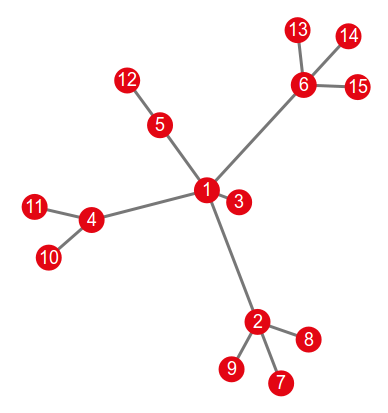
\includegraphics[scale=0.5]{imagenes/familia1.png}
\end{center}
  \caption{Grafo perteneciente a la Familia 1}\label{fig:familia1}
\endminipage\hfill
\minipage{0.5\textwidth}
\begin{center}
  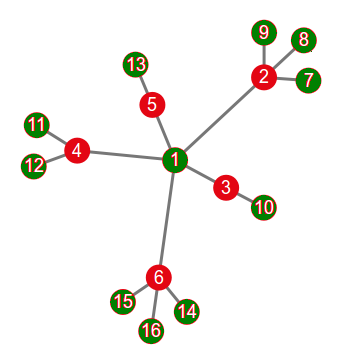
\includegraphics[scale=0.5]{imagenes/familia1-res.png}
\end{center}
  \caption{Solución hallada por nuestra heurística}\label{fig:familia1res}
\endminipage
\end{figure}

\subsubsection*{Familia 2 - Circuitos}

Como miembros de esta familia consideraremos a los circuitos simples.  Para este tipo de grafos, la calidad de la solución hallada por nuestro algoritmo dependerá de la cantidad de vértices que tenga y de la forma en que se hayan rotulado los mismos.

Consideremos un circuito $C_{n}$ y supongamos por un momento que los vértices están rotulados como $v_0,v_1,...,v_{n-1}$ tal que existe una arista entre $v_i$ y $v_j$ cuando $j = (i+1) mod (n)$.

1. Una forma de armar un conjunto independiente maximal $C$ para este grafo podría ser la siguiente:

\begin{itemize}
\item Si $n \equiv 0 (3)$, tomar $C = \{v_i | i \equiv 1 (3)\}$.
\item Si $n \equiv 1 (3)$, tomar $C = \{v_i | i \equiv 1 (3)\} \cup \{v_{n-1}\}$.
\item Si $n \equiv 2 (3)$, tomar $C = \{v_i | i \equiv 1 (3)\}$.
\end{itemize}

2. Veamos que $C$ efectivamente es independiente maximal, y por lo tanto, dominante.

\paragraph*{Independencia:} Cuando $n \equiv 0 (3)$, el conjunto $C$ está formado por los vértices $v_i$ tal que $i \equiv 1 (3)$, por lo cual $v_i$ se comunica con $v_{i-1}$ y con $v_{i+1}$. Como $i-1 \equiv 0 (3)$ y $i+1 \equiv 2 (3)$, entonces los vértices incluidos en $C$ no se comunican entre sí. Cuando $n \equiv 1 (3)$ ó $n \equiv 2 (3)$, todo lo antes escrito también vale, considerando que $v_{n-1}$ (que en ambos casos pertenece a $C$) tiene por vecinos a $v_{n-2}$ y $v_{0}$, y sucede que $0 \equiv 0 (3)$ y $n-2 \equiv 2 (3)$ ó $n-2 \equiv 0 (3)$, por lo cual sigue cumpliéndose la independencia.

\paragraph*{Maximalidad:} Supongamos que $C$ no es maximal, es decir, que podemos incluir al menos un vértice más y seguir teniendo un conjunto independiente. Analicemos los siguientes casos:

\begin{itemize}
	\item Agregar un vértice $v_i$ tal que $i \equiv 1 (3)$.  Pero todos ya forman parte de $C$. ABSURDO.
	\item Agregar un vértice $v_i$ tal que $i \equiv 2 (3)$.  Pero todos se encuentran conectados al vértice $v_{i-1}$ y como en este caso $i-1 \equiv 1(3)$, entonces por definición $v_{i-1} \in C$. ABSURDO.
	\item Agregar un vértice $v_i$ tal que $i \equiv 0 (3)$.  Pero entonces $v_i$ o bien se conecta al vértice $v_{i+1}$ con $i+1 \equiv 1 (3)$ y por lo tanto $v_{i+1} \in C$, o bien $i = n-1$ cuando $n \equiv 1 (3)$ así que también pertenece a $C$. ABSURDO.
\end{itemize}

Luego, $C$ es un conjunto independiente maximal, y por consiguiente, dominante. 

3. Veamos ahora que $C$ también es mínimo (o sea, un CIDM de $C_n$).

Primero, diremos que, dentro de un grafo, un vértice $v$ ``cubre'' a un vértice $w$ o bien cuando $v = w$, o bien cuando $v$ y $w$ son adyacentes. Por lo tanto, un vértice $v$ cubre exactamente a $\delta(v) + 1$ vértices.

Particularmente, dado un CIDM para un determinado grafo $G = (V,E)$, entre todos los vértices pertenecientes a dicho conjunto ``cubren'' a todos los vértices de $G$ (porque es dominante). Notemos además, que dos vértices diferentes del CIDM pueden cubrir a un mismo vértice dentro de $G$ (es decir, pueden tener vecinos en común). Entonces, si tomamos un CIDM $S$ para $G$, y sabiendo que cada vértice $v \in S$ cubre a $\delta(v) + 1$ vértices dentro de $G$, podemos decir que 

\begin{equation*}
\sum_{v \in S} \text{nodos cubiertos por }v = |S| + \sum_{v \in S} \delta(v) \geq |V|
\end{equation*}

Volviendo ahora a nuestro conjunto independiente maximal $C$ del circuito $C_n$ definido anteriormente. En principio, fácilmente vemos su cardinalidad:

\begin{itemize}
	\item Cuando $n \equiv 0 (3), |C| = \frac{n}{3}$.
	\item Cuando $n \equiv 1 (3), |C| = \frac{n-1}{3} + 1$.	
	\item Cuando $n \equiv 2 (3), |C| = \frac{n-2}{3} + 1$.	
\end{itemize}

Para probar que $C$ es un CIDM, supongamos que no lo es.  Es decir, que existe un conjunto independiente y dominante $C'$ con menor cardinalidad que $C$.  Podemos decir que $|C'| = |C| - k$ para algún $k \in [1, |C|)$. Como $C_n$ es un circuito simple, cada vértice tiene grado exactamente 2.  Entonces,

\begin{equation*}
\sum_{v \in C'} \text{nodos cubiertos por }v = |C'| + \sum_{v \in C'} \delta(v) = |C'| + 2|C'| = 3 |C'| = 3(|C| - k) = 3|C| - 3k
\end{equation*}

\begin{itemize}
	\item Cuando $n \equiv 0 (3), 3|C| - 3k = 3\frac{n}{3} - 3k = n-3k < n$ pues $k$ es al menos 1. ABSURDO.
	\item Cuando $n \equiv 1 (3), 3|C| - 3k = 3(\frac{n-1}{3} + 1) - 3k = n+2-3k < n$ pues $k$ es al menos 1. ABSURDO.
	\item Cuando $n \equiv 2 (3), 3|C| - 3k = 3(\frac{n-2}{3} + 1) - 3k = n+1-3k < n$ pues $k$ es al menos 1. ABSURDO.
\end{itemize}

Luego, concluimos que $C$ es un CIDM de $C_n$.

4. Supongamos ahora que vamos armando al conjunto $C$ tomando los nodos $v_i$ de la manera indicada anteriormente, pero de forma secuencial, de menor a mayor valor de $i$. Notamos entonces que:

\begin{itemize}
	\item Cuando $n \equiv 0 (3)$, cada vértice $v_i$ que se incluye en $C$ cubre exactamente 3 vértices ``libres'' (sus dos vecinos y él mismo).
	\item Cuando $n \equiv 1 (3)$, cada vértice $v_i$ que se incluye en $C$ tal que $i \equiv 1 (3)$ también cubre exactamente 3 vértices ``libres'', y por último $v_{n-1}$ sólo se cubre a sí mismo, ya que sus vecinos fueron cubiertos anteriormente por $v_1$ y $v_{n-3}$.
	\item Cuando $n \equiv 2 (3)$, cada vértice $v_i$ que se incluye en $C$ tal que $i \equiv 1 (3)$ también cubre exactamente 3 vértices ``libres'', y por último $v_{n-1}$ se cubre a sí mismo y a $v_{n-2}$, ya que $v_0$ fue cubierto anteriormente por $v_1$.
\end{itemize}

Por lo tanto, podemos decir que al momento de tomar cada vértice de $C$, el mismo califica como nodo ``óptimo''.

5. Definimos ahora la siguiente función $f:V \rightarrow \mathbb{N} \in (0,n]$ para rotular los vértices de $C_n$:

\begin{equation*}
f(v_i) = \begin{cases}
\dfrac{i-1}{3}+1 & \text{si } i \equiv 1 (3)\\\\
k \in (|C|,n] \text{ no utilizado aún} & \text{si no}
\end{cases}
\end{equation*}

6. Por una decisión implementativa, nuestra heurística golosa va tomando secuencialmente los nodos ``óptimos'' en el orden en el que fueron rotulados (o sea que siempre toma el nodo ``óptimo'' con rotulado menor). Entonces, si tomamos un circuito $C_n$ donde los vértices son $v_0,v_1,...,v_{n-1}$ tal que existe una arista entre $v_i$ y $v_j$ cuando $j = (i+1) mod (n)$, podemos formar un conjunto $C$ como se indica en el punto 1, y sabemos por los puntos 2 y 3 que se trata de un CIDM.  Si además, rotulamos los vértices como se indica en el punto 5, podemos ver que, por lo dicho en el punto 4, nuestro algoritmo encuentra una solución exacta, idéntica al conjunto $C$. La Figura \ref{fig:familia2} muestra un ejemplo de circuito rotulado de la manera indicada, y la Figura \ref{fig:familia2res} muestra la respuesta hallada por nuestro algoritmo.

\begin{figure}[!htb]
\minipage{0.5\textwidth}
\begin{center}
  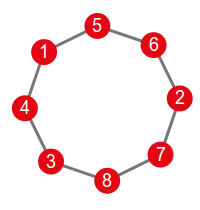
\includegraphics[scale=0.8]{imagenes/faimilia2.png}
\end{center}
  \caption{Circuito simple rotulado ``en orden''}\label{fig:familia2}
\endminipage\hfill
\minipage{0.5\textwidth}
\begin{center}
  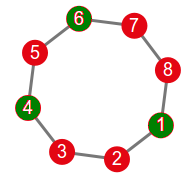
\includegraphics[scale=0.8]{imagenes/faimilia2-resopt.png}
\end{center}
  \caption{Solución hallada por nuestra heurística}\label{fig:familia2res}
\endminipage
\end{figure}


A. Ahora, considerando el circuito $C_n$ inicial, tomemos el siguiente conjunto de vértices $C = \{v_i |(i \equiv 1 (4)) \vee (i \equiv 3 (4))\}$.  Básicamente, tomamos los nodos $v_i$ tal que $i$ es impar.

B. Veamos que $C$ es independiente maximal, y por lo tanto, dominante.

\paragraph*{Independencia:} El conjunto $C$ está formado por los vértices $v_i$ tal que $i \equiv 1 (4)$ ó $i \equiv 3 (4)$. Si $n$ es impar, sabemos que $v_i$ se comunica con $v_{(i-1)}$ y con $v_{(i+1)}$. Si $i \equiv 1 (4)$ entonces $i-1 \equiv 0 (4)$ y $i+1 \equiv 2 (4)$, y si $i \equiv 3 (4)$ entonces $i-1 \equiv 2 (4)$ y $i+1 \equiv 0 (4)$, así que los vértices incluidos en $C$ no se comunican entre sí. Si $n$ es impar, todo lo antes escrito también vale, considerando que $v_{n-1}$ (que pertenece a $C$) tiene por vecinos a $v_{n-2}$ y $v_{0}$, y sucede que $0 \equiv 0 (4)$ y $n-2 \equiv 2 (4)$ ó $n-2 \equiv 0 (4)$, por lo cual sigue cumpliéndose la independencia.

\paragraph*{Maximalidad:} Supongamos que $C$ no es maximal, es decir, que podemos incluir al menos un vértice más y seguir teniendo un conjunto independiente. Analicemos los siguientes casos:

\begin{itemize}
	\item Agregar un vértice $v_i$ tal que $i \equiv 1 (4)$.  Pero todos ya forman parte de $C$. ABSURDO.
	\item Agregar un vértice $v_i$ tal que $i \equiv 3 (4)$.  Pero todos ya forman parte de $C$. ABSURDO.
	\item Agregar un vértice $v_i$ tal que $i \equiv 0 (4)$.  Pero todos se encuentran conectados al vértice $v_{i+1}$ y como en este caso $i+1 \equiv 1(4)$, entonces por definición $v_{i+1} \in C$. ABSURDO.
	\item Agregar un vértice $v_i$ tal que $i \equiv 2 (4)$.  Pero todos se encuentran conectados al vértice $v_{i-1}$ y como en este caso $i-1 \equiv 1(4)$, entonces por definición $v_{i+1} \in C$. ABSURDO.
\end{itemize}

Luego, $C$ es un conjunto independiente maximal, y por consiguiente, dominante. 

C. Veamos ahora que el conjunto $C$ es un conjunto independiente máximo.  Para ello observemos la cardinalidad de $C$ (la cual es trivial dado que sólo tomamos a los vértices $v_i$ con $i$ impar):

\begin{itemize}
	\item Cuando $n$ es par,$|C| = \frac{n}{2}$.
	\item Cuando $n$ es impar, $|C| = \frac{n-1}{2}$.	
\end{itemize}

Para probar que $C$ es un conjunto independiente máximo, supongamos que no lo es.  Es decir, que existe un conjunto independiente maximal $C'$ con mayor cardinalidad que $C$.  Podemos decir que $|C'| = |C| + k$ para algún $k \in [1, (n -|C|))$. Pero dada la cardinalidad de $C$, tener un conjunto con más elementos implicaría que dicho conjunto contiene a más de la mitad de los vértices del grafo, y como se trata de un circuito simple y cada vértice tiene grado 2, obliga a que al menos dos vértices de $C'$ sean adyacentes.  Esto es absurdo puesto que supusimos $C'$ independiente.  Entonces, $C$ es un conjunto independiente máximo.

D. Supongamos ahora que vamos armando al conjunto $C$ tomando los nodos $v_i$ de la manera indicada anteriormente, pero de forma secuencial, de menor a mayor valor de $i$ con $i \equiv 1 (4)$, y luego de menor a mayor valor de $i$ con $i \equiv 3 (4)$. Notamos entonces que:

\begin{itemize}
	\item Cuando tomamos los $v_i$ tal que $i \equiv 1 (4)$, cada uno cubre exactamente 3 vértices ``libres'' (sus dos vecinos y él mismo).
	\item Cuando pasamos a tomar los $v_i$ tal que $i \equiv 3 (4)$ $n \equiv 1 (3)$, cada uno sólo cubre 1 vértice ``libre'' que es él mismo.  Esto sucede porque sus dos vecinos fueron cubiertos anteriormente por los $v_i$ con $i \equiv 1 (4)$.
\end{itemize}

Por lo tanto, podemos decir que al momento de tomar cada vértice de $C$, el mismo califica como nodo ``óptimo''.

E. Definimos ahora la siguiente función $f:V \rightarrow \mathbb{N} \in (0,n]$ para rotular los vértices de $C_n$:

\begin{equation*}
f(v_i) = \begin{cases}
\dfrac{i-1}{4}+1 & \text{si } i \equiv 1 (4)\\\\
\dfrac{i-3}{4}+\left\lfloor \dfrac{n}{4} \right\rfloor + 1 & \text{si } i \equiv 3 (4) \wedge (n \equiv 0 (4) \vee n \equiv 1 (4))\\\\
\dfrac{i-3}{4}+\left\lceil \dfrac{n}{4} \right\rceil + 1 & \text{si } i \equiv 3 (4) \wedge (n \equiv 2 (4) \vee n \equiv 3 (4))\\\\
k \in \left(\dfrac{n}{2},n\right] \text{ no utilizado aún} & \text{si } (i \equiv 0 (4) \vee i \equiv 2 (4)) \wedge (n \equiv 0 (4) \vee n \equiv 2 (4))\\\\
k \in \left(\dfrac{n-1}{2},n\right] \text{ no utilizado aún} & \text{si } (i \equiv 0 (4) \vee i \equiv 2 (4)) \wedge (n \equiv 1 (4) \vee n \equiv 3 (4))\\\\
\end{cases}
\end{equation*}

F. Como hemos decidido nuestra heurística golosa vaya tomando secuencialmente los nodos ``óptimos'' en el orden en el que fueron rotulados, entonces si tomamos un circuito $C_n$ donde los vértices son $v_0,v_1,...,v_{n-1}$ tal que existe una arista entre $v_i$ y $v_j$ cuando $j = (i+1) mod (n)$, podemos formar un conjunto $C$ como se indica en el punto A, y sabemos por los puntos B y C que se trata de un conjunto independiente máximo, y por consiguiente, dominante.  Si además, rotulamos los vértices como se indica en el punto E, podemos ver que, por lo dicho en el punto D, nuestro algoritmo encuentra una solución idéntica al conjunto $C$. 

Hay una excepción para el caso $n \equiv 2 (4)$. En estos casos, el vértice $n-1 \equiv 1 (4)$, pero el vértice $v_{n-1}$ no será tomado por nuestro algoritmo dado que se conecta al vértice $v_0$ que ya fue cubierto por $v_1$ y sólo podría cubrir a su otro vecino y a él mismo como nodos ``libres'', así que en su lugar se tomará al vértice $v_{i-2}$ que puede cubrir a 3 vértices ``libres'' (él mismo, $v_{n-1}$ y $v_{n-3}$, ya que $n-3 \equiv 3 (4)$ y aún no fue tomado). Por consiguiente, al comenzar a tomar a los $v_i$ tales que $i \equiv 3 (4)$, $v_{n-3}$ no será tomado en cuenta ya que no está ``libre''.  Luego, cuando $n \equiv 2 (4)$, la solución hallada por nuestra heurística toma a todos los $v_i$ tal que $i \equiv 1 (4)$ salvo $v_{n-1}$, luego toma a $v_{i-2}$, y finalmente toma a todos los $v_i$ tal que $i \equiv 3 (4)$ salvo $v_{n-3}$.  El tamaño del conjunto hallado, entonces, difiere sólo en una unidad respecto al conjunto planteado en el punto A.

La Figura \ref{fig:familia2bis} muestra un ejemplo de circuito rotulado de la manera indicada, y la Figura \ref{fig:familia2bisres} muestra la respuesta hallada por nuestro algoritmo.

\vspace*{0.3cm}

Para poder comparar las soluciones halladas por nuestra heurística para los rotulados propuestos, aproximaremos la cardinalidad del conjunto encontrado a $\frac{n}{3}$ para el primer caso y $\frac{n}{2}$ para el último, ya que a valores de $n$ muy grandes, la diferencia respecto a $\frac{n-1}{3}+1$ y a $\frac{n-2}{3}+1$ para el primero, y a $\frac{n-1}{2}$ en el segundo, es despreciable.  Entonces podemos decir que la mejor solución para un circuito simple $C_n$ contiene $\frac{n}{3}$ elementos mientras que la peor solución hallada para el mismo circuito contiene $\frac{n}{2}$ elementos.  En otras palabras, para un rotulado como el propuesto en E, el conjunto encontrado por nuestro algoritmo es un $50\%$ peor que el exacto.

\begin{figure}[!htb]
\minipage{0.5\textwidth}
\begin{center}
  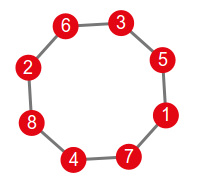
\includegraphics[scale=0.8]{imagenes/faimilia2rename.png}
\end{center}
  \caption{Circuito simple rotulado ``no en orden''}\label{fig:familia2bis}
\endminipage\hfill
\minipage{0.5\textwidth}
\begin{center}
  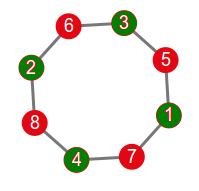
\includegraphics[scale=0.8]{imagenes/faimilia2rename-solnoopt.png}
\end{center}
  \caption{Solución hallada por nuestra heurística}\label{fig:familia2bisres}
\endminipage
\end{figure}



\vspace*{0.6cm}

\subsection{Instancias óptimas.}

\vspace*{0.3cm}

A continuación presentaremos una familia de grafos para la cual nuestra heurística golosa siempre encuentra una solución óptima.

La forma de los grafos pertenecientes a esta familia responde a las siguientes características:

\begin{itemize}
\item Existe un único vértice $v$ que llamaremos ``central'', con grado $\delta(v)$.
\item Para cada vértice $w$ adyacente a $v$, $\delta(w) > \delta(v)$, y sus nodos adyacentes (salvo $v$) tienen grado 1.	
\end{itemize}

Dado que el algoritmo propuesto va tomando en cada paso el nodo ``óptimo'', o sea, aquél que más nodos ``libres'' cubre, en un grafo como el descrito se irá formando el conjunto solución con los vértices adyacentes al nodo ``central'' $v$, y por lo tanto tendrá $\delta(v)$ elementos.  Veamos que esta solución es la mejor. Para esto, veamos que la única diferencia entre esta familia de grafos, y la familia de los grafos estrella, es que el nodo central tiene menor grado que los nodos periféricos. También notemos, que en este caso, nuestra heurística ha tomado la solución óptima descripta para los grafos estrellas. Dado que la explicación sobre por qué esa solución era realmente óptima no tomaba en cuenta el grado del nodo central y de sus periféricos (salvo que implícitamente pedía que estos últimos tengan al menos grado dos, cuestión que en este caso también sucede), podemos usarla para probar que nuestro goloso realmente halla un óptimo.

La Figura \ref{fig:familia3} muestra un ejemplo de grafo perteneciente a esta familia, y la Figura \ref{fig:familia3res} muestra en color verde la solución hallada por nuestro algoritmo.

\begin{figure}[!htb]
\minipage{0.5\textwidth}
\begin{center}
  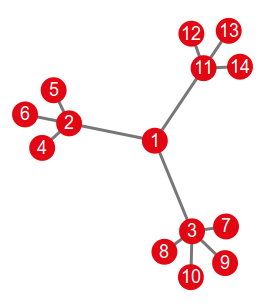
\includegraphics[scale=0.5]{imagenes/familia3.png}
\end{center}
  \caption{Grafo perteneciente a la Familia óptima}\label{fig:familia3}
\endminipage\hfill
\minipage{0.5\textwidth}
\begin{center}
  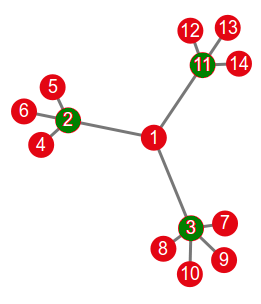
\includegraphics[scale=0.5]{imagenes/familia3-res.png}
\end{center}
  \caption{Solución hallada por nuestra heurística}\label{fig:familia3res}
\endminipage
\end{figure}


\vspace*{0.6cm}

\subsection{Experimentación y gráficos.}

\vspace*{0.3cm}

En esta sección, trataremos de mostrar de manera empírica que nuestro algoritmo posee complejidad cuadrática, y exponer una estimación de la calidad de las soluciones que presenta el mismo.

\subsubsection{Complejidad:}

Para mostrar que nuestro algoritmo tiene complejidad $\mathcal{O}(n^2)$ se generaron 1960 instancias $aleatorias$ con entre 4 y 200 nodos. Luego de correr el algoritmo y tomar las respectivas mediciones de tiempo, se colocaron las mismas en un gráfico al cual se agregó la curva correspondiente a la función $2 \cdot n^2$.  Dicho gráfico se muestra en la Figura \ref{fig:2A}, y como puede apreciarse, todas las mediciones caen por debajo de la curva cuadrática. 

\begin{figure}[htb]
	\begin{center}
    		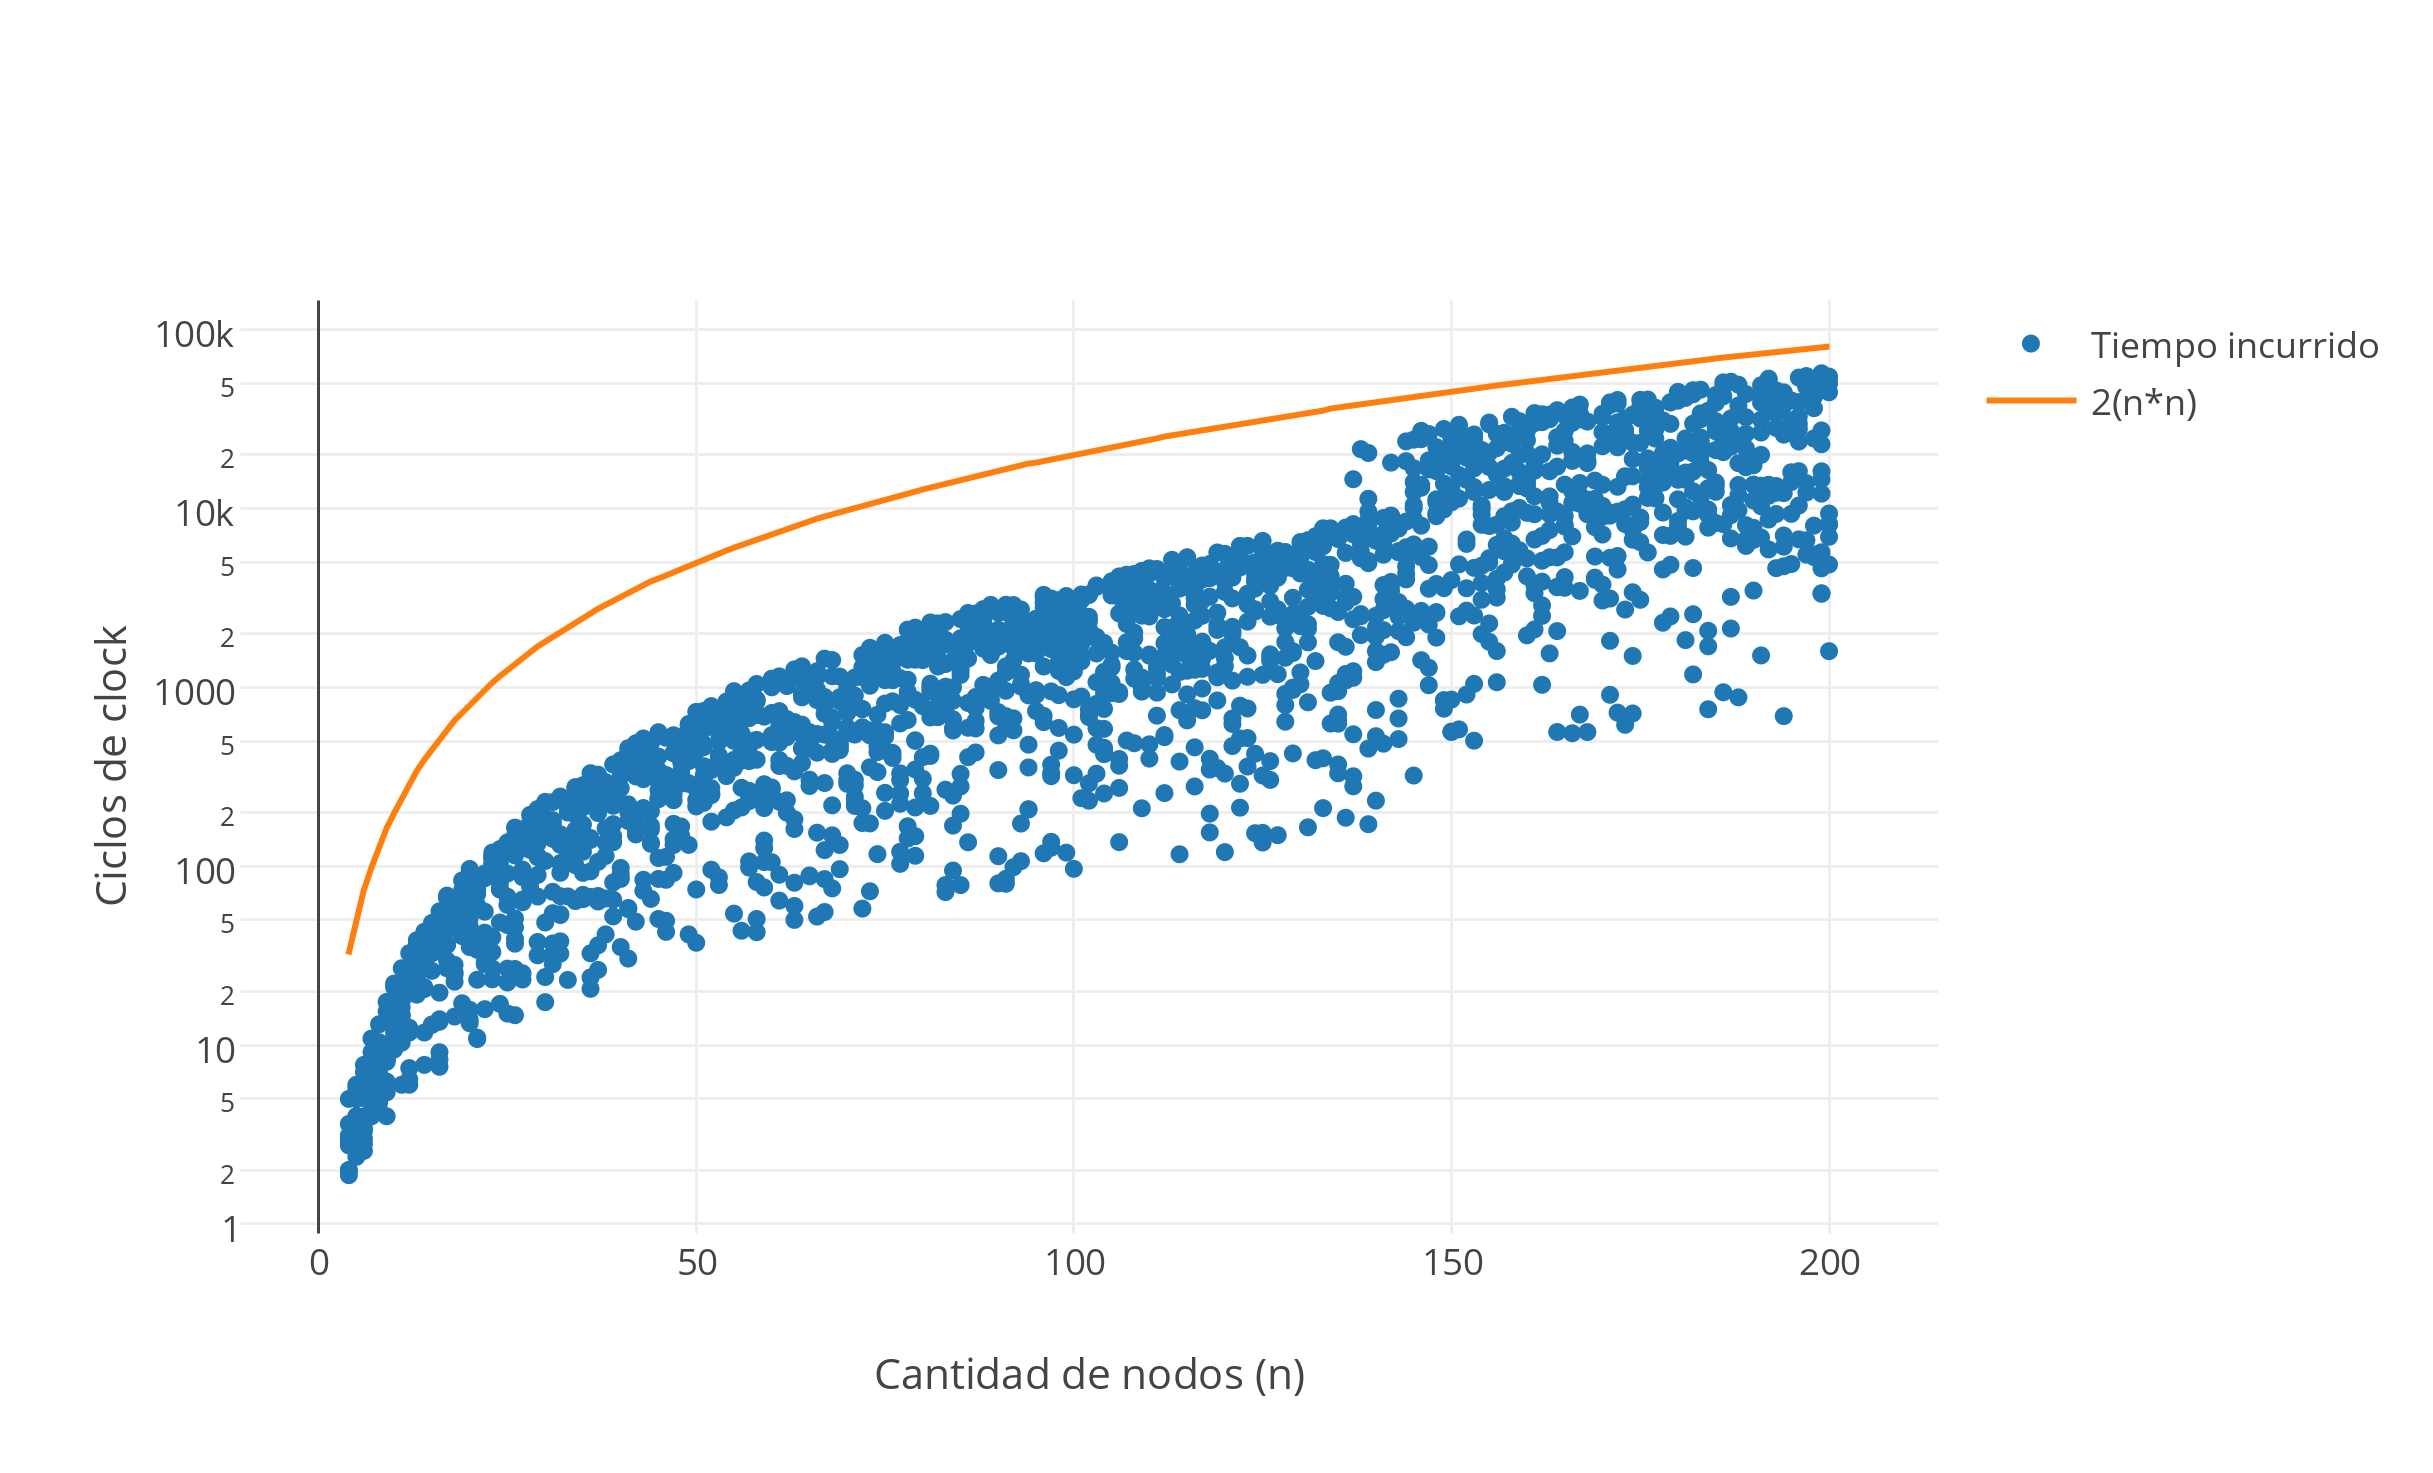
\includegraphics[scale=0.8]{imagenes/goloso-aleatorios.png}
	\end{center}
	\caption{Goloso - Grafos aleatorios\label{fig:2A}}
\end{figure}

\subsubsection{Calidad:}

Para evaluar la calidad de las soluciones obtenidas mediante nuestra heurística, se han generado instancias de tipo $circuito$, $estrella$, $galaxia$ y $aleatorio$.

\paragraph{Circuitos} Se han creado 95 $circuitos$ de entre 5 y 200 nodos.  El orden de los nodos fue aleatorizado para no depender de un rotulado en particular.

La Figura \ref{fig:2B} muestra el tamaño de las soluciones obtenidas en comparación con el tamaño de la solución exacta. Para una cantidad de nodos suficientemente chica, nuestro algoritmo parece tener un error pequeño (en ocasiones nulo), pero a medida que la cantidad de nodos incrementa, el margen de error también parece incrementarse.

\begin{figure}[htb]
	\begin{center}
    		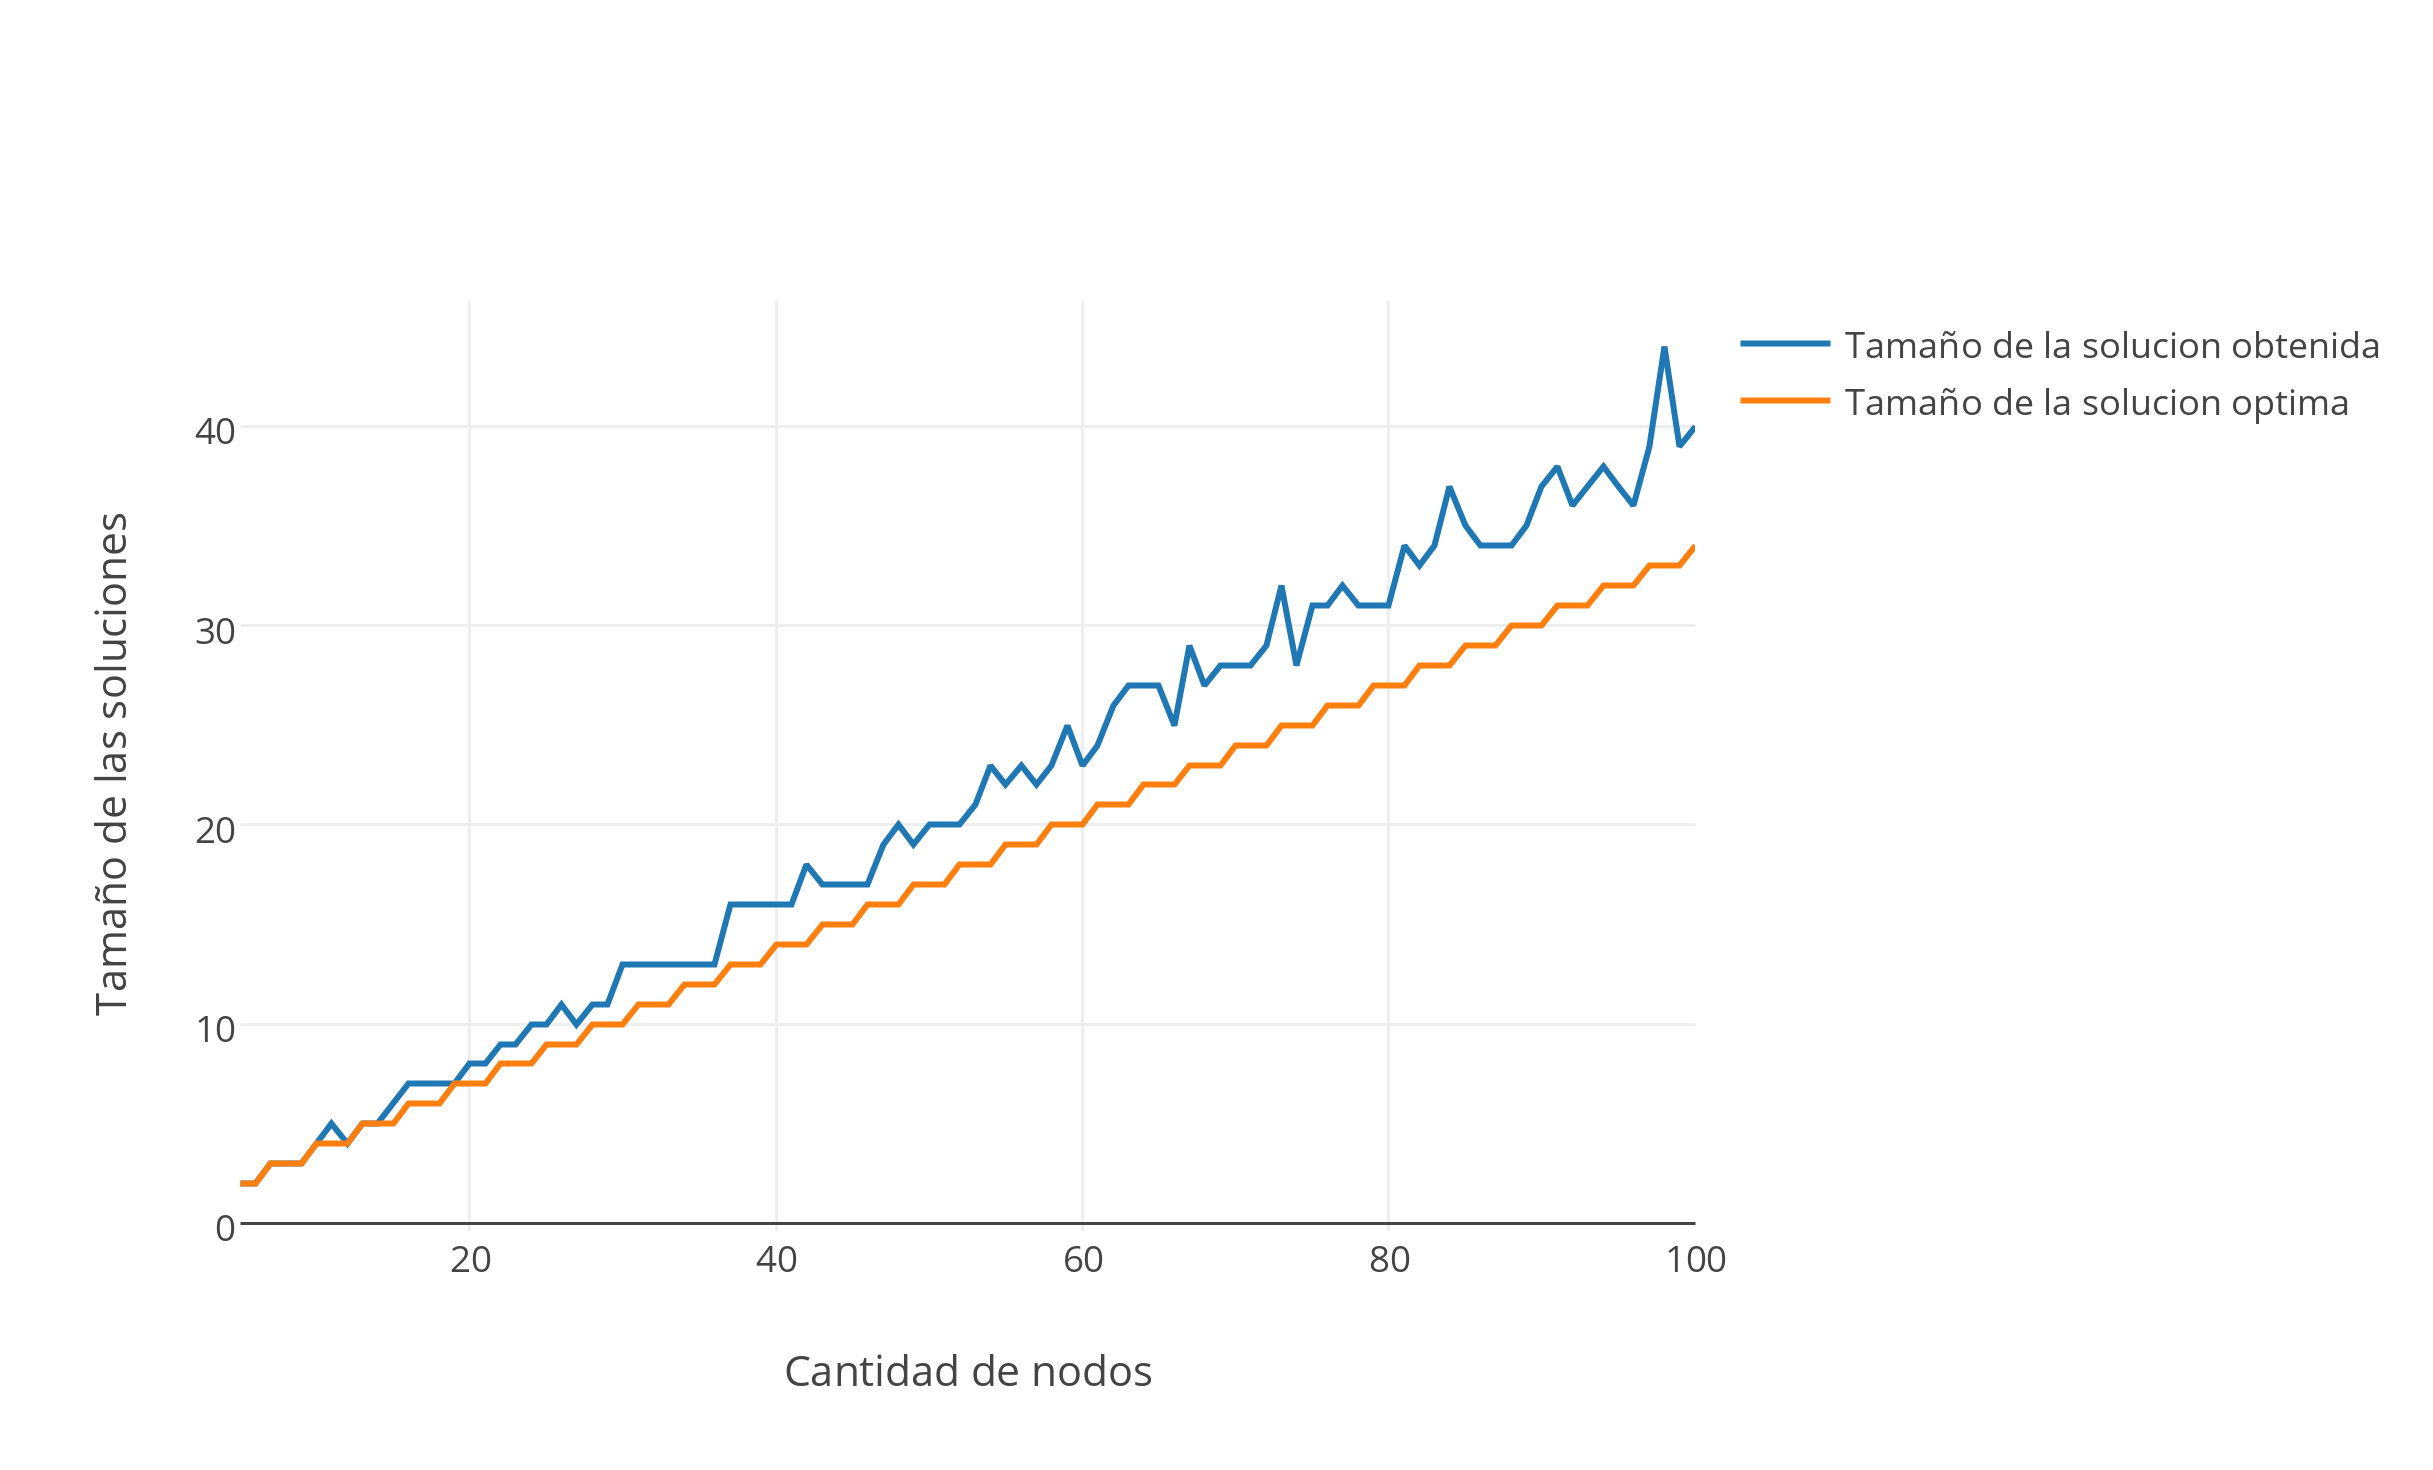
\includegraphics[scale=0.8]{imagenes/goloso-circuito.png}
	\end{center}
	\caption{Goloso - Circuitos \label{fig:2B}}
\end{figure}

\paragraph{Estrella} Se han creado 500 instancias de $estrellas$ de manera que el grado máximo se encuentre entre 10 y 100.

La Figura \ref{fig:2C} muestra el tamaño de las soluciones obtenidas para estas instancias, en comparación con el tamaño de la solución óptima y con la cota superior hallada teóricamente en secciones anteriores. Se puede apreciar que el tamaño de las soluciones efectivamente se ve acotado por el cuadrado del grado máximo, y que además se encuentra mucho más cerca de este valor que del resultado exacto. La experimentación parecería confirmar, entonces, que se trata de una familia de grafos para los cuales nuestra heurística arroja resultados poco precisos.

\begin{figure}[htb]
	\begin{center}
    		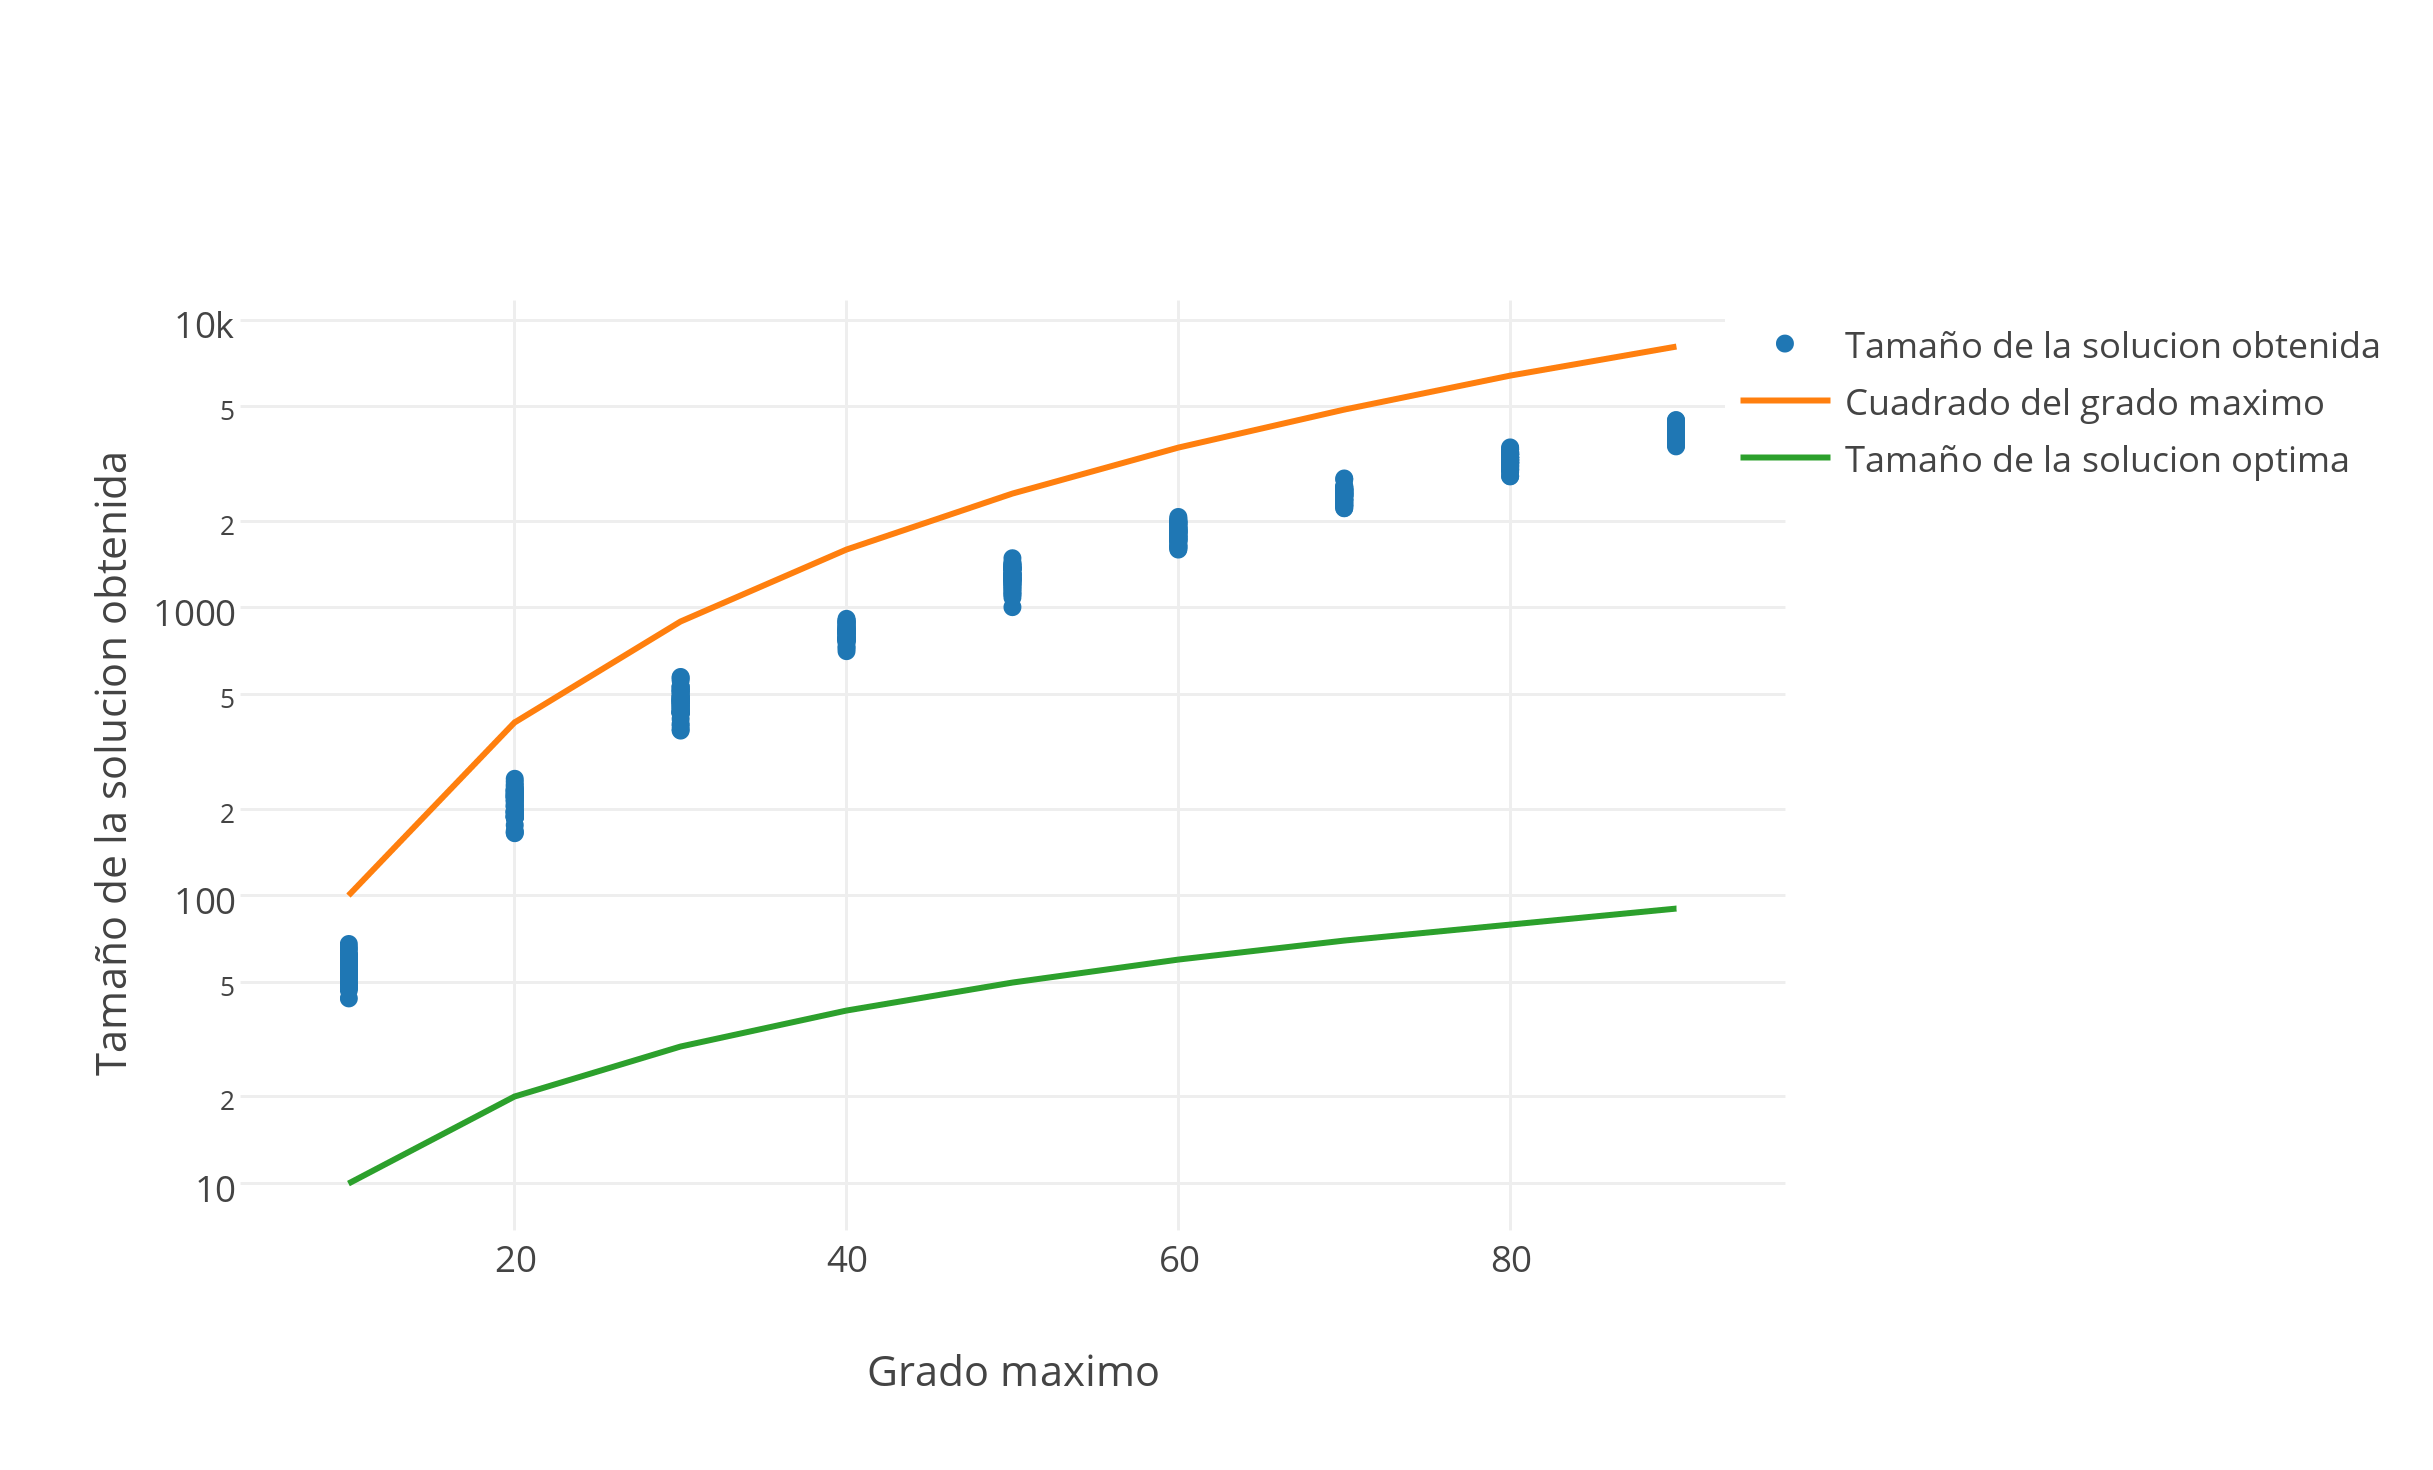
\includegraphics[scale=0.8]{imagenes/goloso-estrella.png}
	\end{center}
	\caption{Goloso - Estrellas \label{fig:2C}}
\end{figure}

\paragraph{Galaxia} Se han creado 500 instancias de $galaxias$ de manera que el grado del nodo central se encuentre entre 5 y 100.

Para estos casos, el tamaño de las soluciones obtenidas coinciden exactamente con el tamaño de la solución exacta. Esto indicaría que se trata de una familia de grafos para los cuales nuestra heurística arroja resultados exactos.

\paragraph{Aleatorios} Se han creado 120 instancias $aleatorias$ con entre 4 y 15 nodos, de manera de poder comparar los resultados de nuestra heurística con los resultados del algoritmo exacto. El porcentaje de respuestas coincidentes entre la heurística y el exacto fue de $89.167\%$. Podemos decir, bajo esta experimentación, que si bien el algoritmo no es exacto, proporciona una buena respuesta en el caso general.

\vspace*{0.6cm}

\newpage
\section{Heurística de Busqueda Local}
\subsection{Desarrollo de la idea.}

\vspace*{0.3cm}

La heurística de búsqueda local que hemos diseñado, parte de una solución inicial, y a partir de ahí irá encontrando nuevas soluciones ``vecinas''.  Si una solución ``vecina'' resulta ser mejor, es decir, es un conjunto independiente maximal con menos elementos que la solución anterior, entonces la reemplazará.  Estos pasos se repitirán hasta que se encuentre una solución que no pueda mejorarse, es decir, una solución óptima local.

Se analizarán dos posibles soluciones iniciales:

\begin{itemize}
\item La solución hallada por el algoritmo goloso presentado anteriormente.
\item Una solución hallada de la siguiente manera: tomando los nodos del grafo en cierto orden, si el nodo actual no forma parte del conjunto solución ni es adyacente a un nodo del conjunto solución, entonces agregarlo al mismo; en caso contrario, avanzar al siguiente nodo.
\end{itemize}

Para cada solución factible $S$, se define $N(S)$ como el conjunto de ``soluciones vecinas'' de $S$.  Plantearemos dos ``vecindades'' posibles para las soluciones.  

\begin{itemize}
\item {\bf Vecindad 1:} Una solución $S' \in N(S)$ si y sólo si puede obtenerse intercambiando tres nodos de $S$ por dos nodos que no pertenecía a $S$.  Es decir, para $u,v,w \in S$, y $x,y$ nodos del grafo original tal que $x \not \in S$ y $y \not \in S$, definimos $S' = S - \{u,v,w\} + \{x,y\}$ y decimos que $S'$ es ``vecina'' de $S$ si y sólo si $S'$ es un conjunto independiente maximal del grafo original. La Figura \ref{fig:vec1} es un ejemplo de solución ``vecina'' conisderando a la Figura \ref{fig:solinicial} como solución inicial para el grafo de la Figura \ref{fig:estrellita}.  En este caso, se han quitado los nodos 1, 8 y 11 para agregar los nodos 3 y 5.
\item {\bf Vecindad 2:} Una solución $S' \in N(S)$ si y sólo si puede obtenerse agregando a $S$ un nodo del grafo original que no pertenezca a $S$, y quitando todos los nodos de $S$ adyacentes a este nuevo nodo.  Es decir, para $v$ un nodo del grafo original tal que $v \not \in S$, y $A \subseteq S$ tal que para todo $w \in S$, si $w$ es adyacente a $v$ entonces $w \in A$, definimos $S' = S - A + \{v\}$ y decimos que $S'$ es ``vecina'' de $S$ si y sólo si $S'$ es un conjunto independiente maximal del grafo original.  La Figura \ref{fig:vec2} es un ejemplo de solución ``vecina'' conisderando a la Figura \ref{fig:solinicial} como solución inicial para el grafo de la Figura \ref{fig:estrellita}.  En este caso, se ha agregado el nodo 2 y se han quitado los nodos 1, 6 y 7.
\end{itemize}

 
\begin{figure}[!htb]
\minipage{0.5\textwidth}
\begin{center}
  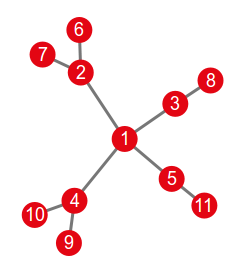
\includegraphics[scale=0.8]{imagenes/estrellita.png}
\end{center}
  \caption{Ejemplo de grafo}\label{fig:estrellita}
\endminipage\hfill
\minipage{0.5\textwidth}
\begin{center}
  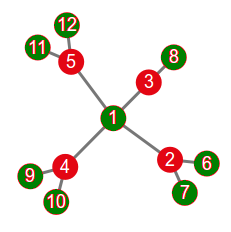
\includegraphics[scale=0.8]{imagenes/estrellitasolinicial.png}
\end{center}
  \caption{Posible solución inicial}\label{fig:solinicial}
\endminipage
\vspace*{0.3cm}
\minipage{0.5\textwidth}%
\begin{center}
  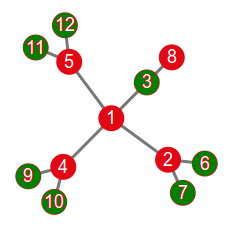
\includegraphics[scale=0.8]{imagenes/estrellitavec1.png}
\end{center}
  \caption{Solución vecina según Vecindad 1}\label{fig:vec1}
\endminipage\hfill
\minipage{0.5\textwidth}
\begin{center}
  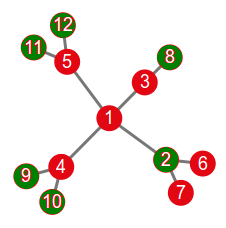
\includegraphics[scale=0.8]{imagenes/estrellitavec2.png}
\end{center}
  \caption{Solución vecina según Vecindad 2}\label{fig:vec2}
\endminipage
\end{figure}
 
 
\vspace*{0.6cm}

%\newpage

\subsection{Análisis de complejidad de una iteración.}

Para analizar la complejidad del algoritmo en este caso, tendremos que hacer una división en dos casos, con mejorador1 y con mejorador2.
Debemos señalar que conseguir la solución inicial no formará parte del análisis de complejidad dado que es un factor externo, por no estar incluido dentro de una iteración del algoritmo.

En el caso de hacer uso de mejorador1, el procedimiento a realizar en una iteración consiste en obtener un grupo de 3 nodos (esto se hace con 3 iteraciones distintas sobre los elementos de la solución, siendo $\mathcal{O}(n)$ cada iteración y llegando a un costo posible de $\mathcal{O}(n^3)$). Por cada posible combinación de estos 3 nodos, se modifican ciertas variables internas para simular la eliminación de estos elementos (toma $3\mathcal{O}(n)$ ya que implica recorrer los vecinos de estos 3 nodos) y se buscan 2 candidatos entre sus vecinos (uniendo los conjuntos de vecinos de los 3 nodos y eliminando los repetidos), mediante 2 iteraciones anidadas sobre el conjunto de vecinos y verificando si resultan viables ($\mathcal{O}(1)$ la verificación y $\mathcal{O}(n^2)$ encontrar los 2 candidatos, en caso de que los haya). En caso de que se cumplan las condiciones para modificar la solución actual, termina la iteración, de lo contrario, se deshacen las modificaciones realizadas ($3\mathcal{O}(n)$) y termina la iteración.

Con esta información, y siendo $T(n)$ la complejidad de nuestro algoritmo, tenemos:

\begin{equation*}
\begin{array}{l}
T(n) = \mathcal{O}(n^3) * \mathcal{O}(n^2) + 3\mathcal{O}(n) + 3\mathcal{O}(n) \\
T(n) = \mathcal{O}(n^5) + 6\mathcal{O}(n) \\
T(n) = \mathcal{O}(n^5)
\end{array}
\end{equation*}

En el caso de utilizar mejorador2, el procedimiento es distinto. Partimos buscando nodos que se relacionen con al menos dos nodos de la solución inicial (preguntar por cada nodo nos toma $\mathcal{O}(n)$). Por cada nodo que cumpla, se actualizan variables relacionadas con ese nodo para simular su incorporación a la solución (para esto se requiere recorrer los vecinos de ese nodo con costo $\mathcal{O}(n)$). Luego revisamos si incorporando el nodo previamente seleccionado llegamos a una solución válida ($\mathcal{O}(n)$), de ser así, quitamos los nodos que se relacionan con éste, modificamos variables para seguir teniendo en cuenta el cambio realizado ($\mathcal{O}(n)$) y terminamos la iteración. En caso contrario, terminamos la iteración (al no modificar las variables del otro caso, estas se verán reseteadas en la siguiente iteración).

En este caso, siendo $T(n)$ la complejidad de nuestro algoritmo, tenemos:

\begin{equation*}
\begin{array}{l}
T(n) = \mathcal{O}(n) * \mathcal{O}(n) + \mathcal{O}(n) + \mathcal{O}(n)\\
T(n) = \mathcal{O}(n^2) + 2\mathcal{O}(n) \\
T(n) = \mathcal{O}(n^2)
\end{array}
\end{equation*}

\vspace*{0.3cm}

\begin{figure}
\begin{codebox}
\Procname{$\proc{CIDM_busqueda}(int$ $mej)$}
\li $cidm\_sol \leftarrow$ lista de nodos de una solución inicial
\li $res \leftarrow |cidm\_sol|$
\li \While haya mejoras y la última solución tenga más de un nodo
\li \Do 
		\If $mej == 1$
\li 		\Then {\sc mejorador1}($cidm\_sol,res$)
\li 		\Else {\sc mejorador2}($cidm\_sol,res$)
		\End
	\End
\end{codebox}
\caption{Heurística de búsqueda local para CIDM}\label{code:busqueda}
\end{figure}
%\FloatBarrier


\begin{figure}
\begin{codebox}
\Procname{$\proc{Mejorador1}(lista\_nodos$ $cidm\_sol,int$ $res)$} 
\li \For cada grupo de 3 de nodos en $cidm\_sol$
\li \Do 
		``sacar'' los 3 nodos
\li 		\For cada par de vecinos $n1,n2$ de estos nodos
\li 		\Do 
			\If $n1$ y $n2$ quedaron ``libres'' y no son adyacentes
\li			\Then
				``agregar'' $n1$ y $n2$
\li 				\If se forma una solución válida
\li 				\Then salir del ciclo
				\End
			\End
		\End
\li 		\If se encontró una solución mejor
\li 		\Then
			actualizar $cidm\_sol$
\li 			actualizar $res$
\li 			\Return
		\End
	\End
\li \Return
\end{codebox}
\caption{Pseudocódigo de la mejora 1}\label{code:mej1}
\end{figure}
%\FloatBarrier



\begin{figure}
\begin{codebox}
\Procname{$\proc{Mejorador2}(lista\_nodos$ $cidm\_sol,int$ $res)$} 
\li \For cada nodo $n$
\li \Do 
		\If $n$ se conecta con al menos dos nodos de $cidm\_sol$
\li 		\Then 
			\For cada nodo de $cidm\_sol$ que se conecta a $n$
\li 			\Do 
				``sacar'' el nodo
\li 				\If se forma una solución válida
\li 				\Then salir del ciclo
				\End
			\End
\li 			\If se encontró una solución mejor
\li 			\Then
				actualizar $cidm\_sol$
\li 				actualizar $res$
\li 				\Return
			\End
		\End
	\End
\li \Return
\end{codebox}
\caption{Pseudocódigo de la mejora 2}\label{code:mej2}
\end{figure}
%\FloatBarrier


\vspace*{0.6cm}
%\newpage
\subsection{Experimentación y gráficos.}

\vspace*{0.3cm}


\subsubsection{Test 1}
\vspace*{0.3cm}

\vspace*{0.6cm}
%\newpage

\subsubsection{Test 2}



\newpage
\section{Metaheurística de GRASP}
\subsection{Desarrollo de la idea.}

\vspace*{0.3cm}

GRASP (Greedy Randomized Adaptative Search Procedure) es una combinación entre una heurística golosa ``aleatorizada'' y un procedimiento de búsqueda local.  La idea es la siguiente:

\begin{codebox}
\li \While no se alcance el {\it criterio de terminación}
\li \Do 
		Obtener una solución inicial mediante una {\it heurística golosa aleatorizada}.
\li 		Mejorar la solución mediante búsqueda local.
\li 		Recordar la mejor solución obtenida hasta el momento.
	\End
\end{codebox}

Como criterios de terminación, analizaremos dos casos particulares:

\begin{itemize}
\item Se realizaron $50$ iteraciones.
\item Se realizaron $10$ iteraciones sin encontrar una solución mejor.
\end{itemize}

En cuanto a la heurística golosa aleatorizada, hemos continuado con la idea del algoritmo goloso descrito anteriormente, con la variación de que, en cada paso, se genera una Lista Restricta de Candidatos (RCL) y se elige aleatoriamente un candidato de esa lista.  Analizaremos dos posibles maneras de construir dicha RCL:

\begin{enumerate}
\item Hallar al mejor candidato, es decir, el nodo que hemos definido como óptimo, y colocar en la RCL los nodos candidatos cuya cantidad de vecinos ``libres'' sea no menor a un $10 \%$ de la cantidad de vecinos ``libres'' del mejor candidato.
\item Hallar al mejor candidato y colocar en la RCL los $5$ mejores candidatos, es decir, los $5$ nodos que más nodos ``libres'' cubran.
\end{enumerate}

\vspace*{0.6cm}

\newpage
\subsection{Experimentación y gráficos.}

\vspace*{0.3cm}

En esta sección trataremos de encontrar, entre las posibles combinaciones de criterios de parada y listas restrictas de candidatos explicadas anteriormente, aquella que tenga el mejor balance entre calidad de solución y performance. Se ha elegido utilizar la segunda vecindad explicada en la sección de busqueda local, debido a su balance entre tiempo de ejecución y solución obtenida.  

Para facilitar la lectura, nombraremos a cada configuracón de la siguiente manera:

\begin{itemize}
	\item {\bf Configuración 1:} Utiliza como como criterio de parada realizar 10 iteraciones sin mejoras, y el primer RCL .
	\item {\bf Configuración 2:} Utiliza como como criterio de parada realizar 10 iteraciones sin mejoras, y el segundo RCL .
	\item {\bf Configuración 3:} Utiliza como como criterio de parada realizar 50 iteraciones, y el primer RCL .
	\item {\bf Configuración 4:} Utiliza como como criterio de parada realizar 50 iteraciones, y el segundo RCL .

\end{itemize}

Plantearemos entonces, experimentos que nos permitan observar cómo se desenvuelve nuestro algoritmo con cada configuración, y con los resultados, tratar de elegir una de ellas. Para ello se ha decidido evaluar instancias de tipo $circuito$, $estrella$, $galaxia$ y $aleatorio$.
 
\subsubsection{Circuitos}

Se generaron 20 $circuitos$ con entre 10 y 30 nodos.  El orden de los nodos fue aleatorizado para no depender de un rotulado en particular.

\paragraph{Performance} 

El gráfico obtenido con las mediciones de tiempo es el que se muestra en la Figura \ref{fig:4A}.

\begin{figure}[htb]
	\begin{center}
    		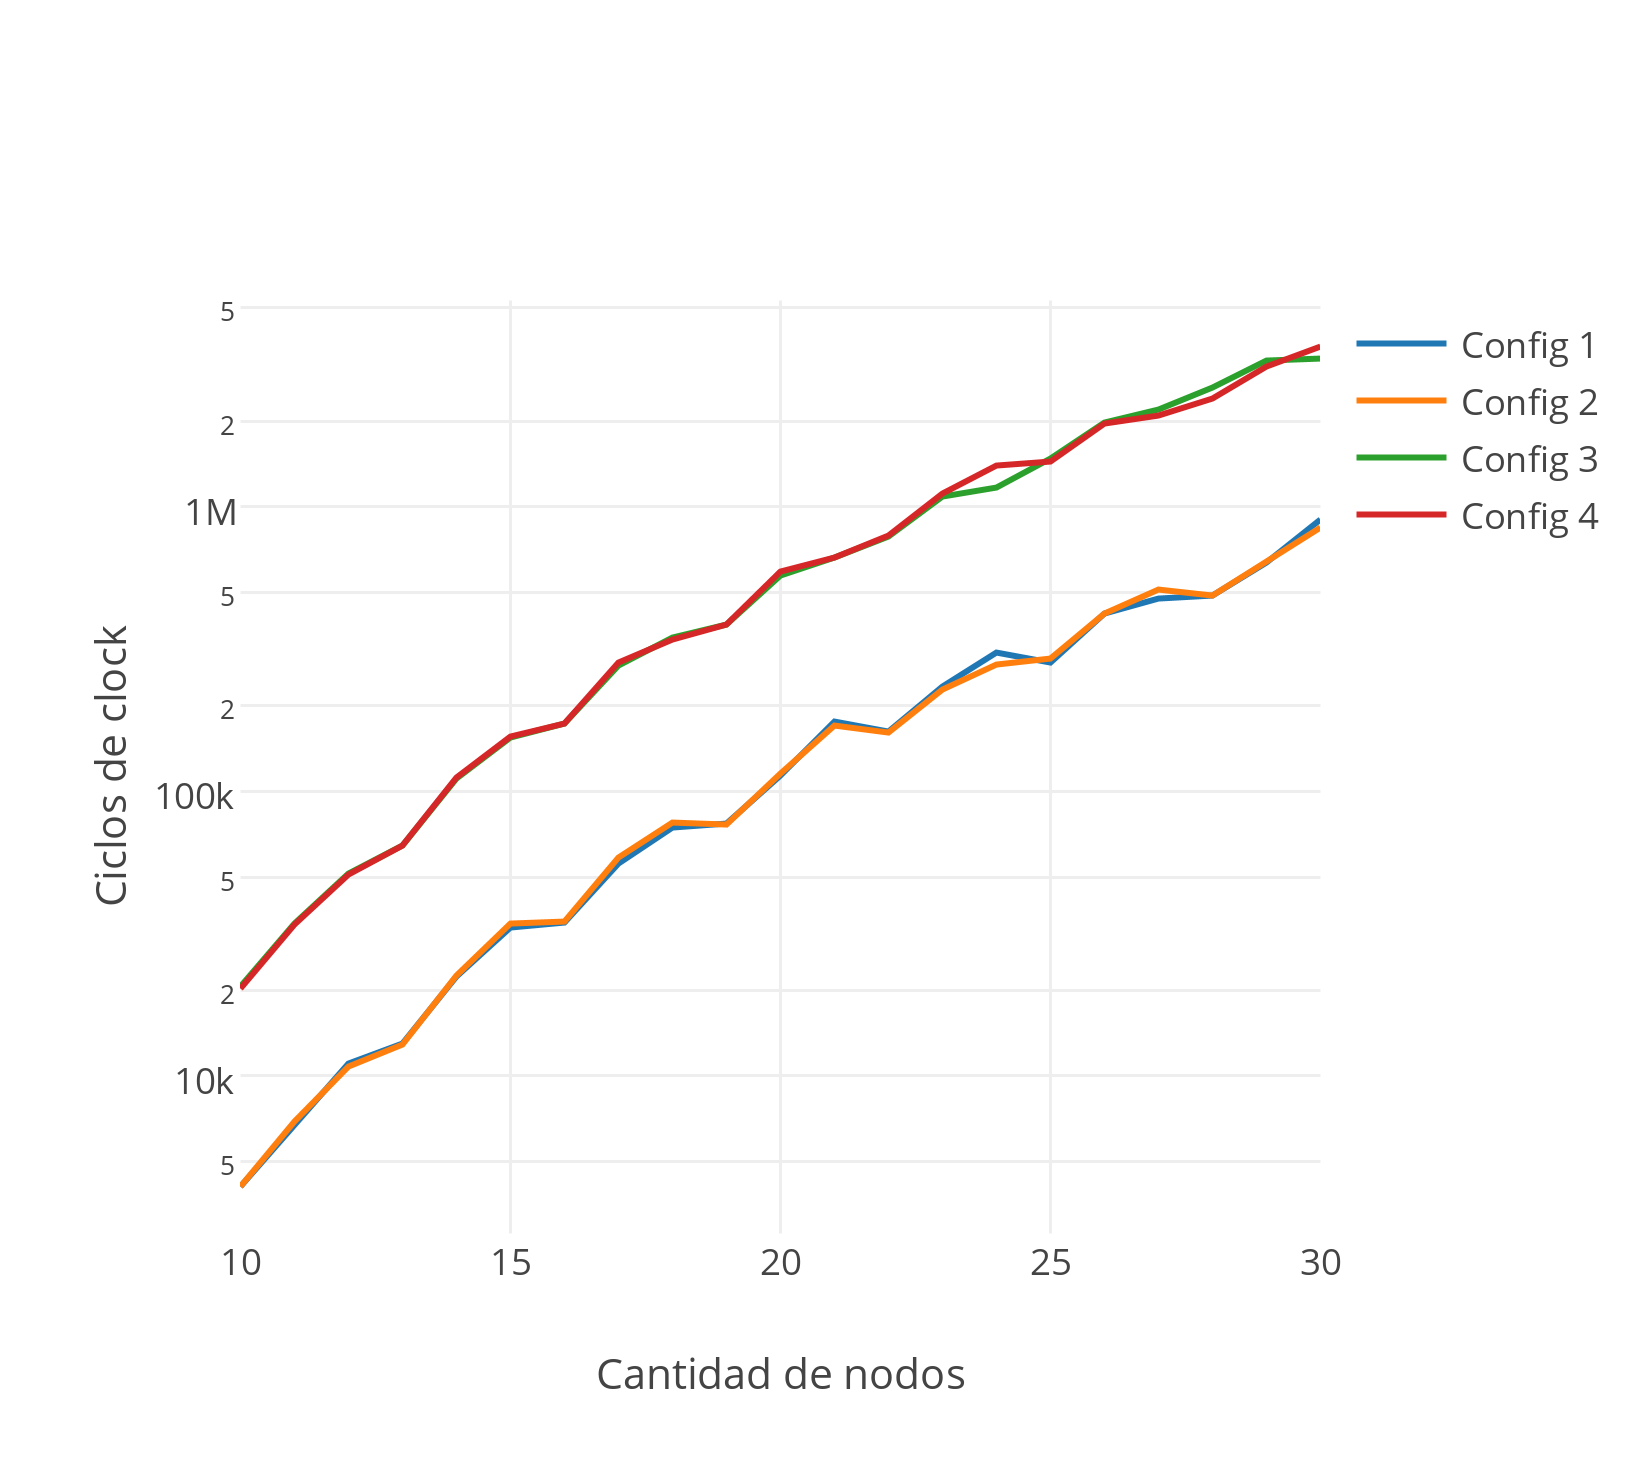
\includegraphics[scale=0.8]{imagenes/grasp-circuitos-tiempo.png}
	\end{center}
	\caption{GRASP - Circuitos}\label{fig:4A}
\end{figure}
%\FloatBarrier

La Figura parece indicar que aquellas configuraciones que utilizan el criterio de parada de 50 iteraciones(desde ahora llamado segundo criterio) tienen un desempeño peor que aquellas que utilizan el criterio de parada de 10 iteraciones sin mejora(desde ahora llamado primer criterio). Entre las configuraciones que utilizan el mismo criterio de parada, no parece ser posible indicar de manera precisa cual RCL optimiza más el tiempo de corrida del algoritmo.

\paragraph{Calidad} Se ha comparado el tamaño de la solución hallada con el tamaño de la solución exacta.  Los porcentajes de desaciertos sobre el total de instancias evaluadas son los siguientes:

\begin{verbatim}
Configuración 1: 0%
Configuración 2: 0%
Configuración 3: 0%
Configuración 4: 0%
\end{verbatim}

Pareciera entonces, que sin importar la configuración, para este tipo de grafos GRASP no provoca errores.
\subsubsection{Estrellas}

Se generaron 30 grafos $estrellas$ con grado máximo entre 5 y 7.

\paragraph{Performance}

La Figura \ref{fig:4B} muestra los resultados obtenidos respecto al tiempo de ejecución. Nuevamente, las configuraciones que utilizan el primer criterio de parada muestran un desempeño considerablemente mejor en términos de performance que aquellas que utilizan el segundo.
Se puede destacar, que la configuración 1 tiene el menor tiempo de ejecución.

\begin{figure}[htb]
	\begin{center}
    		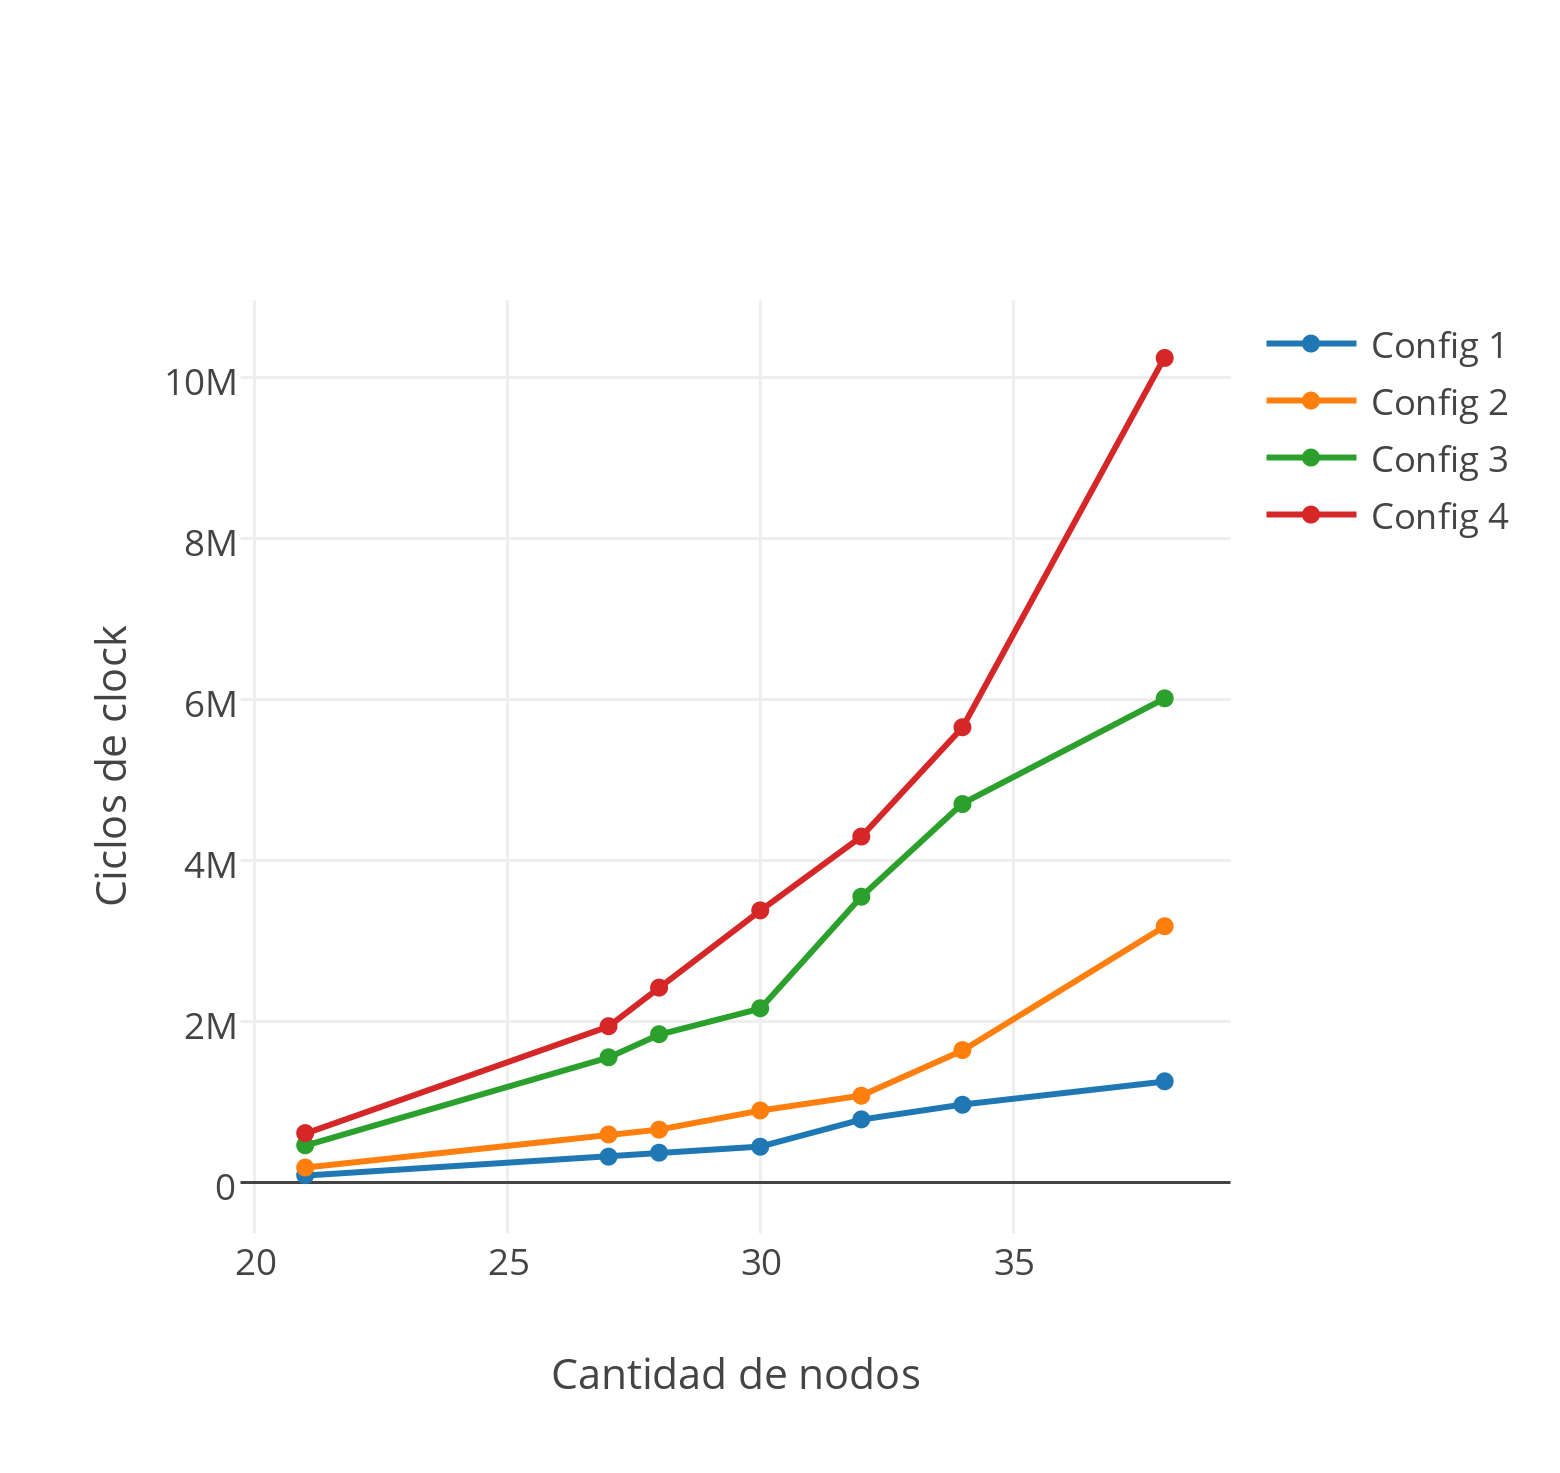
\includegraphics[scale=0.8]{imagenes/grasp-estrellas-tiempo.png}
	\end{center}
	\caption{GRASP - Estrellas}\label{fig:4B}
\end{figure}
%\FloatBarrier

\paragraph{Calidad} Se ha comparado el tamaño de la solución obtenida con el tamaño de la solución exacta. Los porcentajes de desaciertos sobre el total de instancias evaluadas son los siguientes:

\begin{verbatim}
Configuración 1: 3.34%
Configuración 2: 63.34%
Configuración 3: 0%
Configuración 4: 13.34%
\end{verbatim}

Podemos observar como la configuración 1 y 3 tienen las mejores tasas de acierto, llegando esta última a no cometer errores. Cabe destacar que la configuración 2 tiene para este tipo de grafos, un porcentaje de desaciertos muy amplio.

\subsubsection{Galaxias}

Se generaron 20 grafos $galaxia$ con entre 7 y 38 nodos.

\paragraph{Performance}

La Figura \ref{fig:4C} muestra los resultados obtenidos respecto al tiempo de ejecución. Aquí, las configuracion 1 es claramente la de mejor performance mientras que la 4 es claramente la de peor tiempo de ejecución. A priori, no podemos determinar según este gráfico quien tiene un mejor desempeño entre las configuraciones 2 y 3. 

\begin{figure}[htb]
	\begin{center}
    		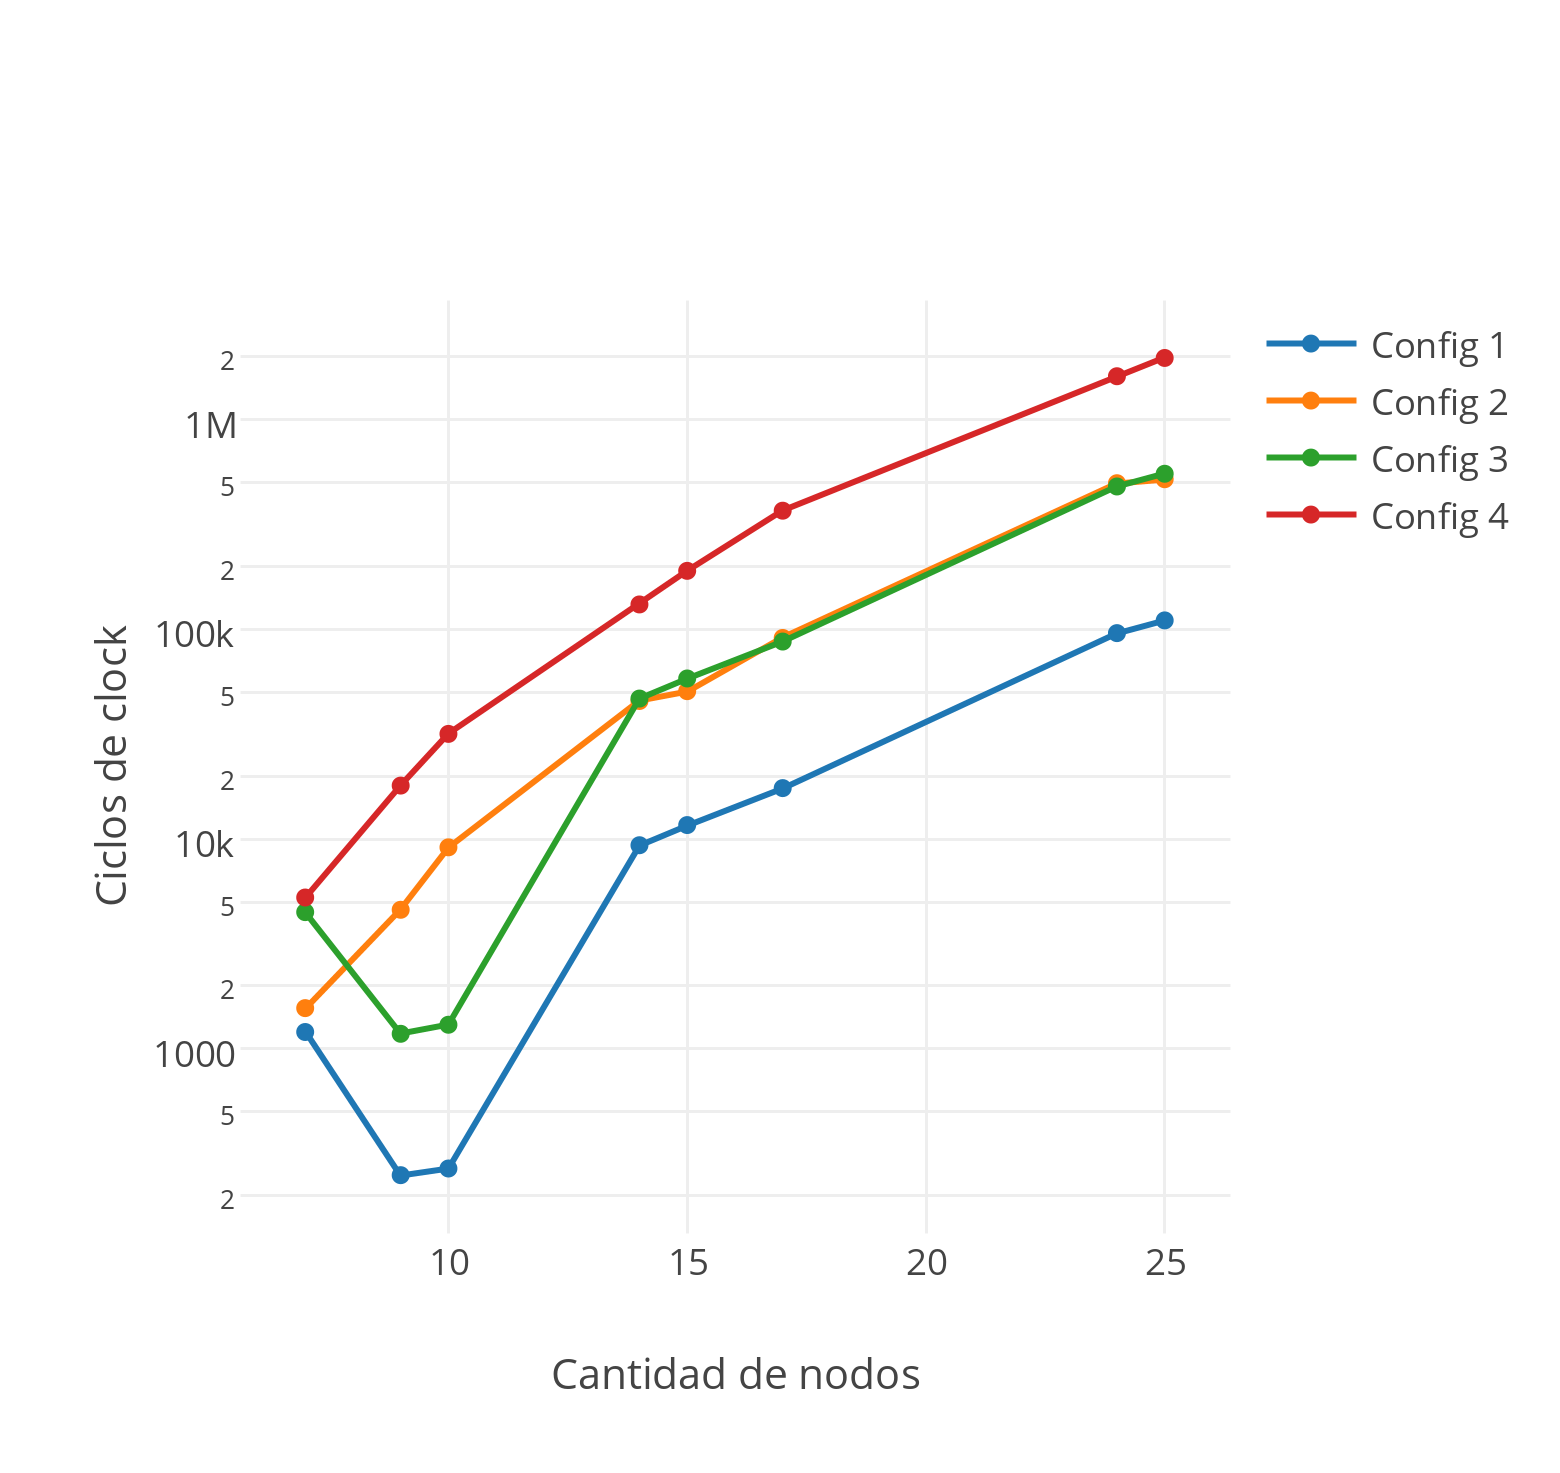
\includegraphics[scale=0.8]{imagenes/grasp-galaxias-tiempos.png}
	\end{center}
	\caption{GRASP - Galaxias}\label{fig:4C}
\end{figure}
%\FloatBarrier

\paragraph{Calidad} 
Se ha comparado el tamaño de la solución obtenida con el tamaño de la solución exacta. Los porcentajes de desaciertos sobre el total de instancias evaluadas son los siguientes:

\begin{verbatim}
Configuración 1: 0%
Configuración 2: 50%
Configuración 3: 0%
Configuración 4: 10%
\end{verbatim}

Podemos observar como las configuraciones 1 y 3 no tuvieron errores, como la configuración 4 vuelve a tener un error aceptable, y como la configuración 2 vuelve a tener una tasa de aciertos muy baja

\subsubsection{Aleatorios}

Para estos experimentos se han generado dos sets de instancias $aleatorias$. Uno contiene 120 grafos de entre 4 y 15 nodos, para poder contrastar con el algoritmo exacto (sólo se utilizara para la parte de calidad). El otro contiene 210 grafos de entre 10 y 30 nodos, que si bien no serán comparadas con el algoritmo exacto, posibilitará apreciar los tiempos de ejecución más ampliamente y tener una idea más general respecto a la calidad de las soluciones obtenidas.

\paragraph{Performance} La Figura \ref{fig:4D} muestra los resultados obtenidos respecto al tiempo de ejecución. Podemos apreciar que las configuraciones que utilizan el primer criterio de parada tienen un desempeño peor que las otras, y entre las configuraciones que utilizan el segundo criterio, la configuración 1 parecería mostrarse como la más óptima.

\begin{figure}[htb]
	\begin{center}
    		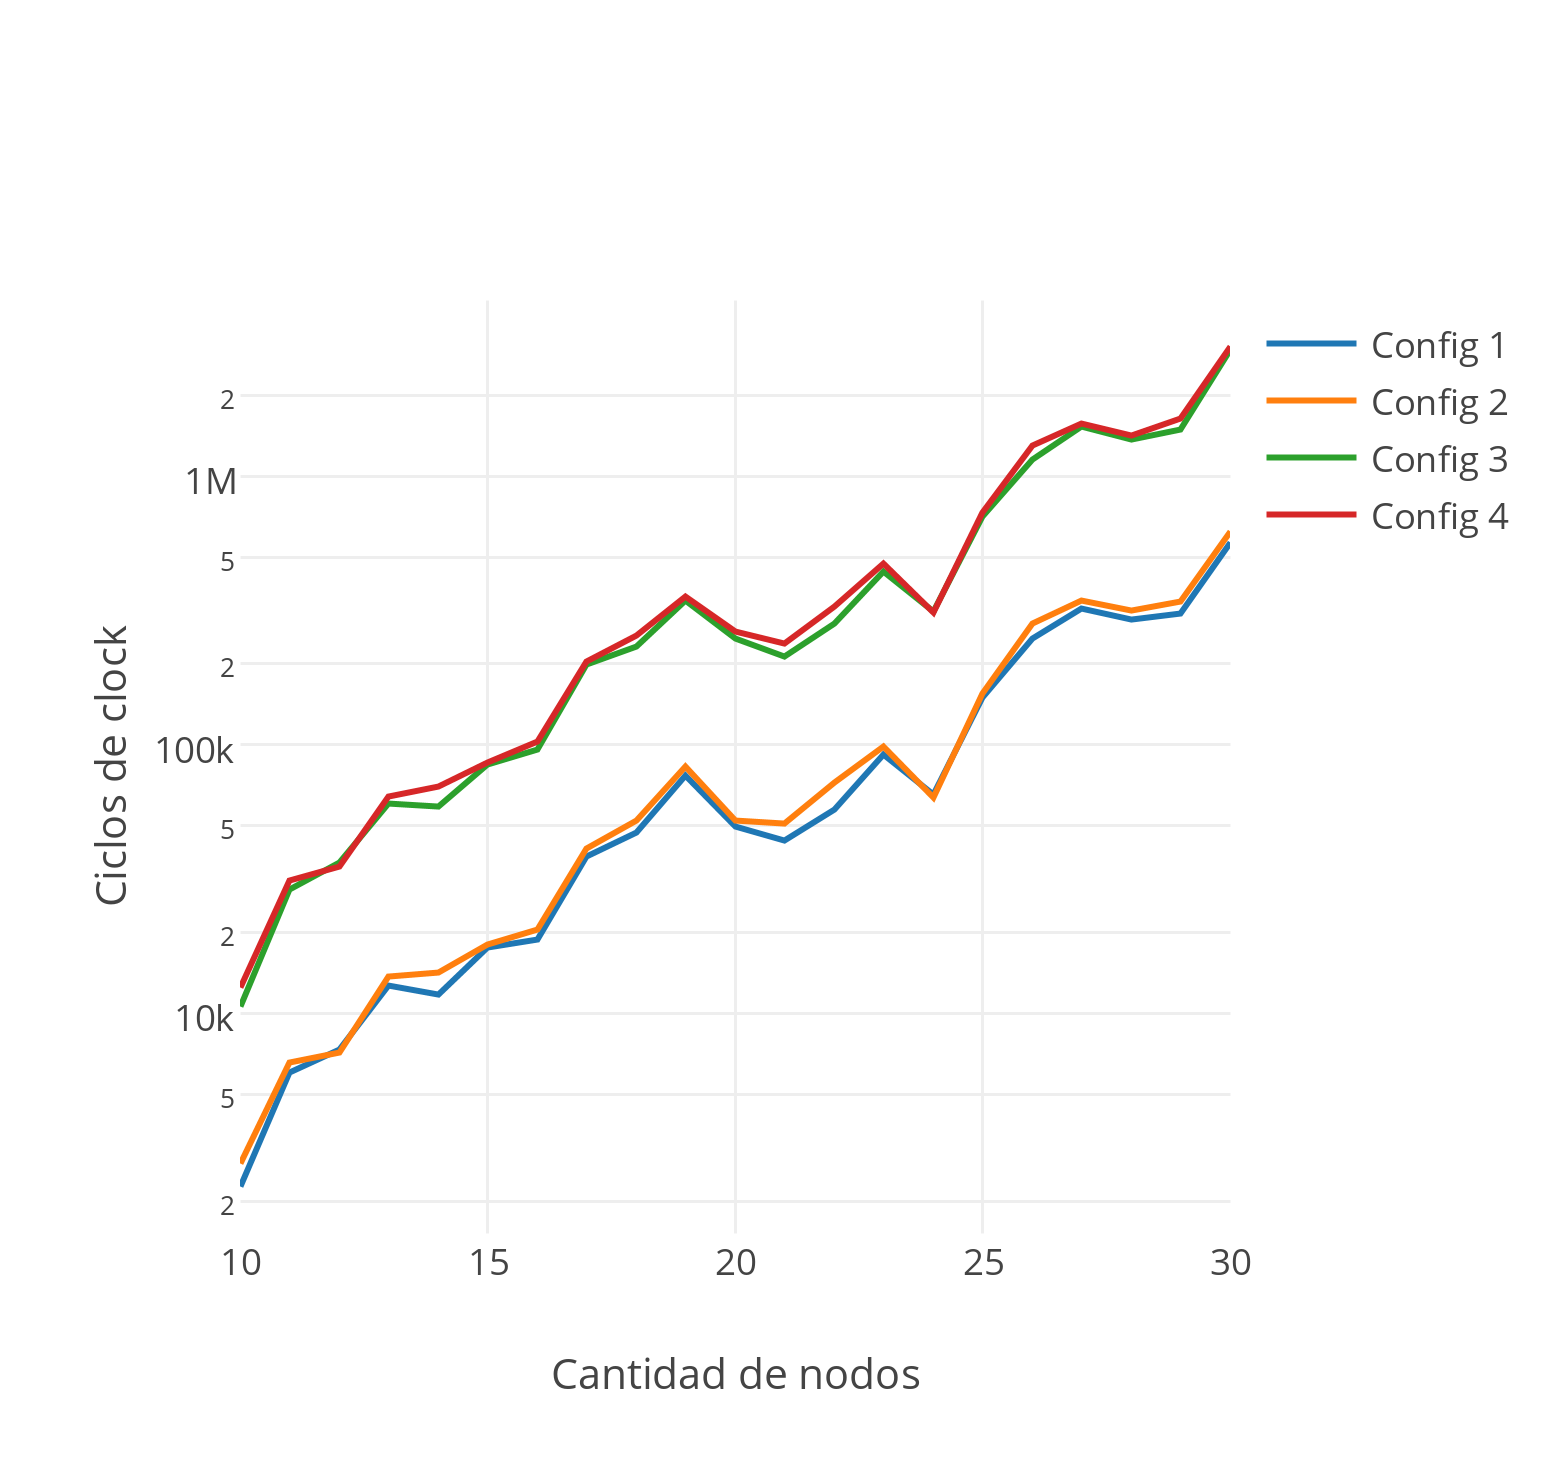
\includegraphics[scale=0.8]{imagenes/grasp-aleatorios-tiempo.png}
	\end{center}
	\caption{GRASP - Aleatorios}\label{fig:4D}
\end{figure}
%\FloatBarrier

\paragraph{Calidad} 

\subparagraph{Set 1} Se ha comparado el tamaño de la solución obtenida con el tamaño de la solución exacta.  Los porcentajes de desaciertos sobre el total de instancias evaluadas son los siguientes:

\begin{verbatim}
Configuración 1: 1.667%
Configuración 2: 0.833%
Configuración 3: 0%
Configuración 4: 0%
\end{verbatim}

Podemos observar que todas las configuraciones tienen una tasa de error muy baja, destacando la 3 y 4 que no tienen errores.

\subparagraph{Set 2} Como por el tamaño de estas instancias se dificulta la comparación con el algoritmo exacto, se consideró como la solución ``óptima'' en cada caso el menor valor obtenido entre las cuatro configuraciones, y se registró, para cada una, la cantidad de instancias en las que no se logró dicho valor. Los porcentajes de estos ``desaciertos'' sobre el total de instancias evaluadas son los siguientes:

\begin{verbatim}
Configuración 1: 1.90%
Configuración 2: 1.43%
Configuración 3: 0.48%
Configuración 4: 0.48%
\end{verbatim}

Podemos notar nuevamente como en el set 1, tasas de error muy bajas, destacando que las configuraciones 3 y 4 ahora tienen algún error.

\subsubsection{Conclusiones} 

Luego de realizar este análisis para distintas instancias, podemos observar que, en lo que respecta a la calidad de las soluciones obtenidas, la configuracion 3 es la que logra obtener mejores resultados. Cabe destacar que si bien para las familias analizadas la configuración 2 arrojo muchos desaciertos, para casos generales esto no sucede. Por otro lado, las configuraciones que utilizan el segundo criterio, requieren un tiempo de ejecución considerablemente mayor que aquellas que utilizan el primero.  Por este motivo, si bien la Configuración 3 es la que se muestra mejor en calidad, decidimos considerar a la Configuración 1 como la que mejor balancea calidad y performance. Notece, que si bien la configuración 2 tiene mejor calidad para aleatorios, configuración 1 no tiene calidad mucho peor para estos casos, tiene una considerable mejor calidad para las familias estudiadas, y es ligeramente más optimo en tiempo.

%\newpage
%\section{Comparación de los distintos métodos}
%\subsection{Experimentación y gráficos.}

\vspace*{0.3cm}

En esta sección trataremos de encontrar, entre las posibles combinaciones de criterios de parada y listas restrictas de candidatos explicadas anteriormente, aquella que tenga el mejor balance entre calidad de solución y performance. Se ha elegido utilizar la segunda vecindad explicada en la sección de busqueda local, debido a su balance entre tiempo de ejecución y solución obtenida.  

Para facilitar la lectura, nombraremos a cada configuracón de la siguiente manera:

\begin{itemize}
	\item {\bf Configuración 1:} Utiliza como como criterio de parada realizar 10 iteraciones sin mejoras, y el primer RCL .
	\item {\bf Configuración 2:} Utiliza como como criterio de parada realizar 10 iteraciones sin mejoras, y el segundo RCL .
	\item {\bf Configuración 3:} Utiliza como como criterio de parada realizar 50 iteraciones, y el primer RCL .
	\item {\bf Configuración 4:} Utiliza como como criterio de parada realizar 50 iteraciones, y el segundo RCL .

\end{itemize}

Plantearemos entonces, experimentos que nos permitan observar cómo se desenvuelve nuestro algoritmo con cada configuración, y con los resultados, tratar de elegir una de ellas. Para ello se ha decidido evaluar instancias de tipo $circuito$, $estrella$, $galaxia$ y $aleatorio$.
 
\subsubsection{Circuitos}

Se generaron 20 $circuitos$ con entre 10 y 30 nodos.  El orden de los nodos fue aleatorizado para no depender de un rotulado en particular.

\paragraph{Performance} 

El gráfico obtenido con las mediciones de tiempo es el que se muestra en la Figura \ref{fig:4A}.

\begin{figure}[htb]
	\begin{center}
    		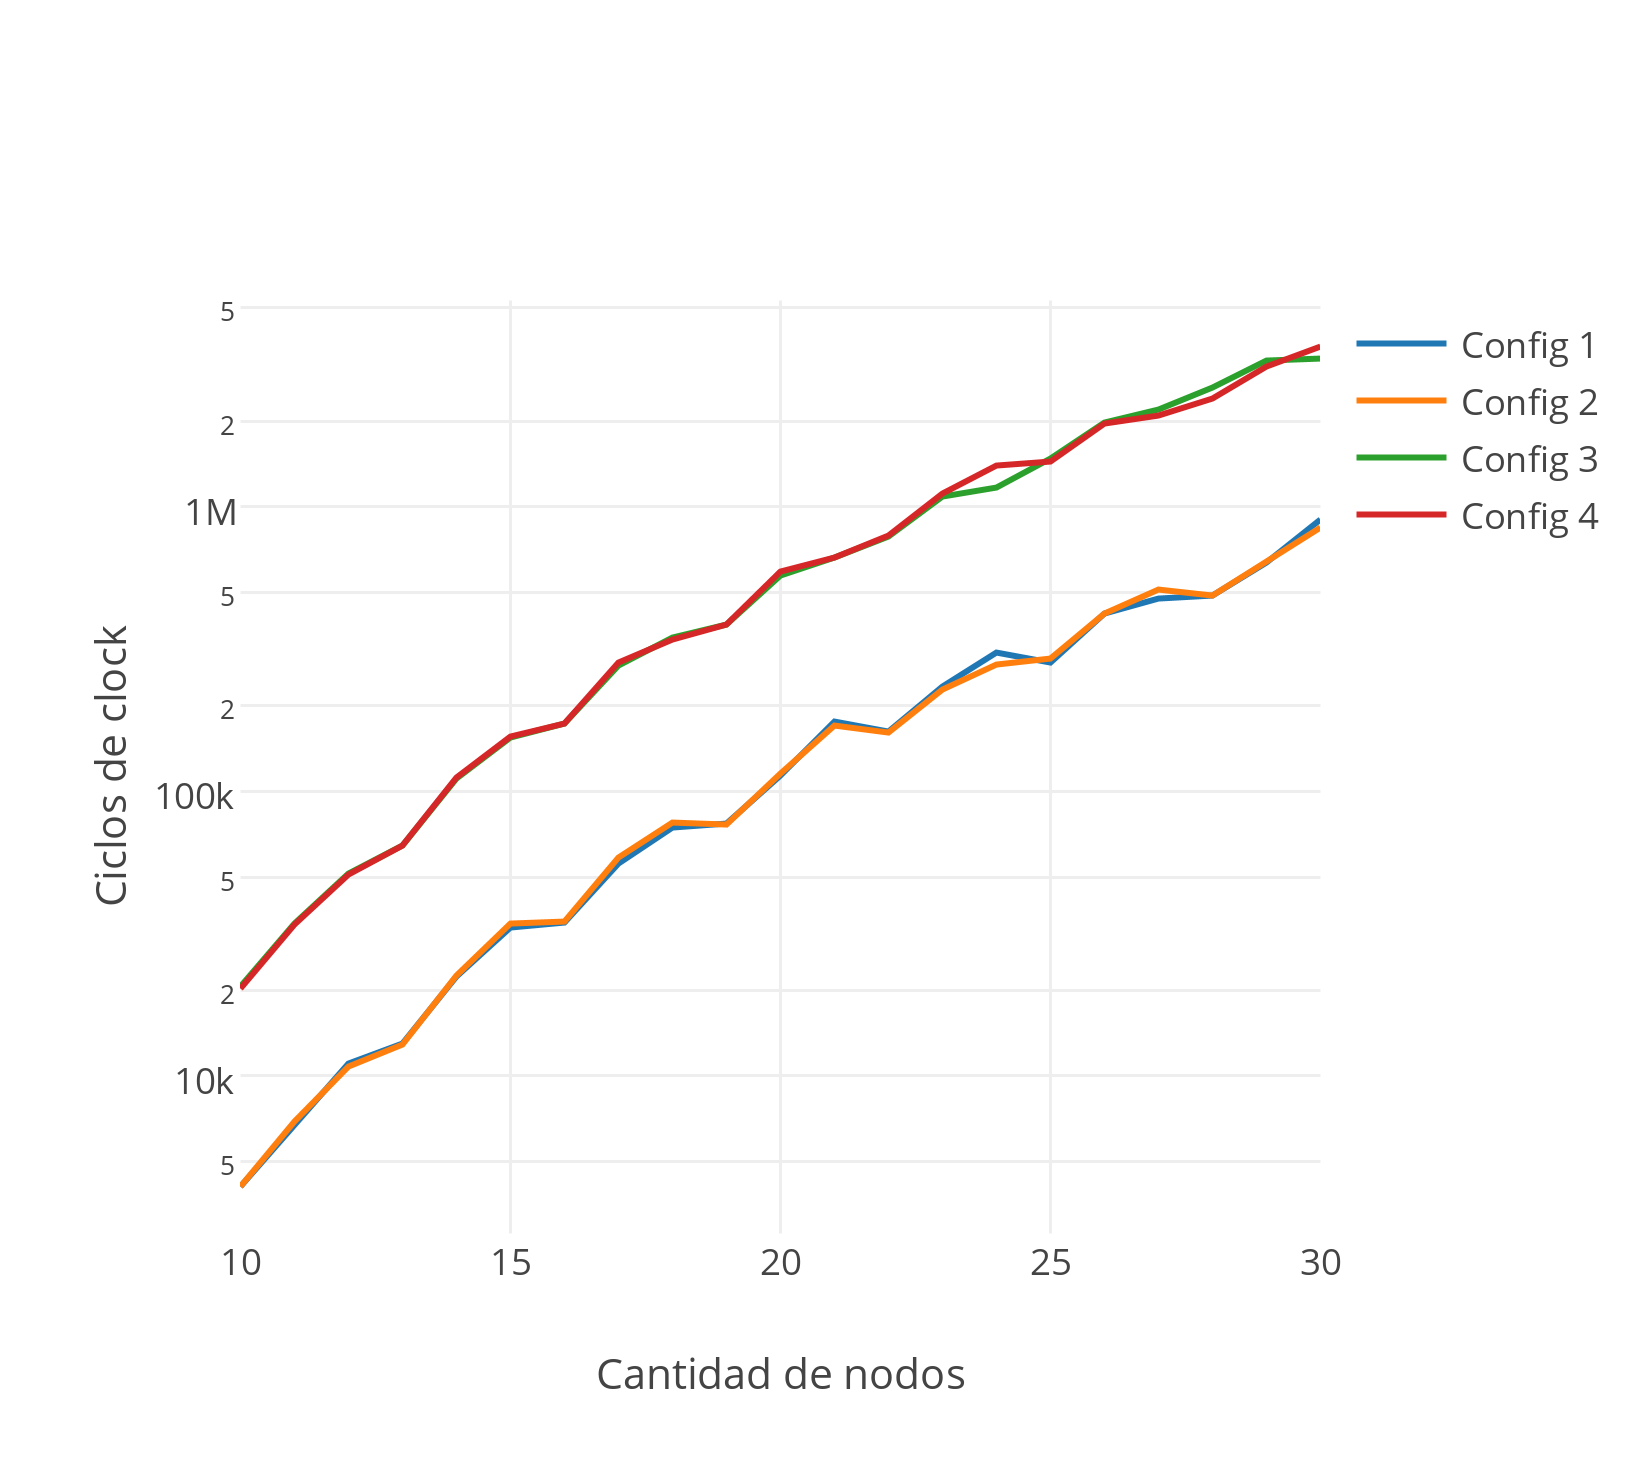
\includegraphics[scale=0.8]{imagenes/grasp-circuitos-tiempo.png}
	\end{center}
	\caption{GRASP - Circuitos}\label{fig:4A}
\end{figure}
%\FloatBarrier

La Figura parece indicar que aquellas configuraciones que utilizan el criterio de parada de 50 iteraciones(desde ahora llamado segundo criterio) tienen un desempeño peor que aquellas que utilizan el criterio de parada de 10 iteraciones sin mejora(desde ahora llamado primer criterio). Entre las configuraciones que utilizan el mismo criterio de parada, no parece ser posible indicar de manera precisa cual RCL optimiza más el tiempo de corrida del algoritmo.

\paragraph{Calidad} Se ha comparado el tamaño de la solución hallada con el tamaño de la solución exacta.  Los porcentajes de desaciertos sobre el total de instancias evaluadas son los siguientes:

\begin{verbatim}
Configuración 1: 0%
Configuración 2: 0%
Configuración 3: 0%
Configuración 4: 0%
\end{verbatim}

Pareciera entonces, que sin importar la configuración, para este tipo de grafos GRASP no provoca errores.
\subsubsection{Estrellas}

Se generaron 30 grafos $estrellas$ con grado máximo entre 5 y 7.

\paragraph{Performance}

La Figura \ref{fig:4B} muestra los resultados obtenidos respecto al tiempo de ejecución. Nuevamente, las configuraciones que utilizan el primer criterio de parada muestran un desempeño considerablemente mejor en términos de performance que aquellas que utilizan el segundo.
Se puede destacar, que la configuración 1 tiene el menor tiempo de ejecución.

\begin{figure}[htb]
	\begin{center}
    		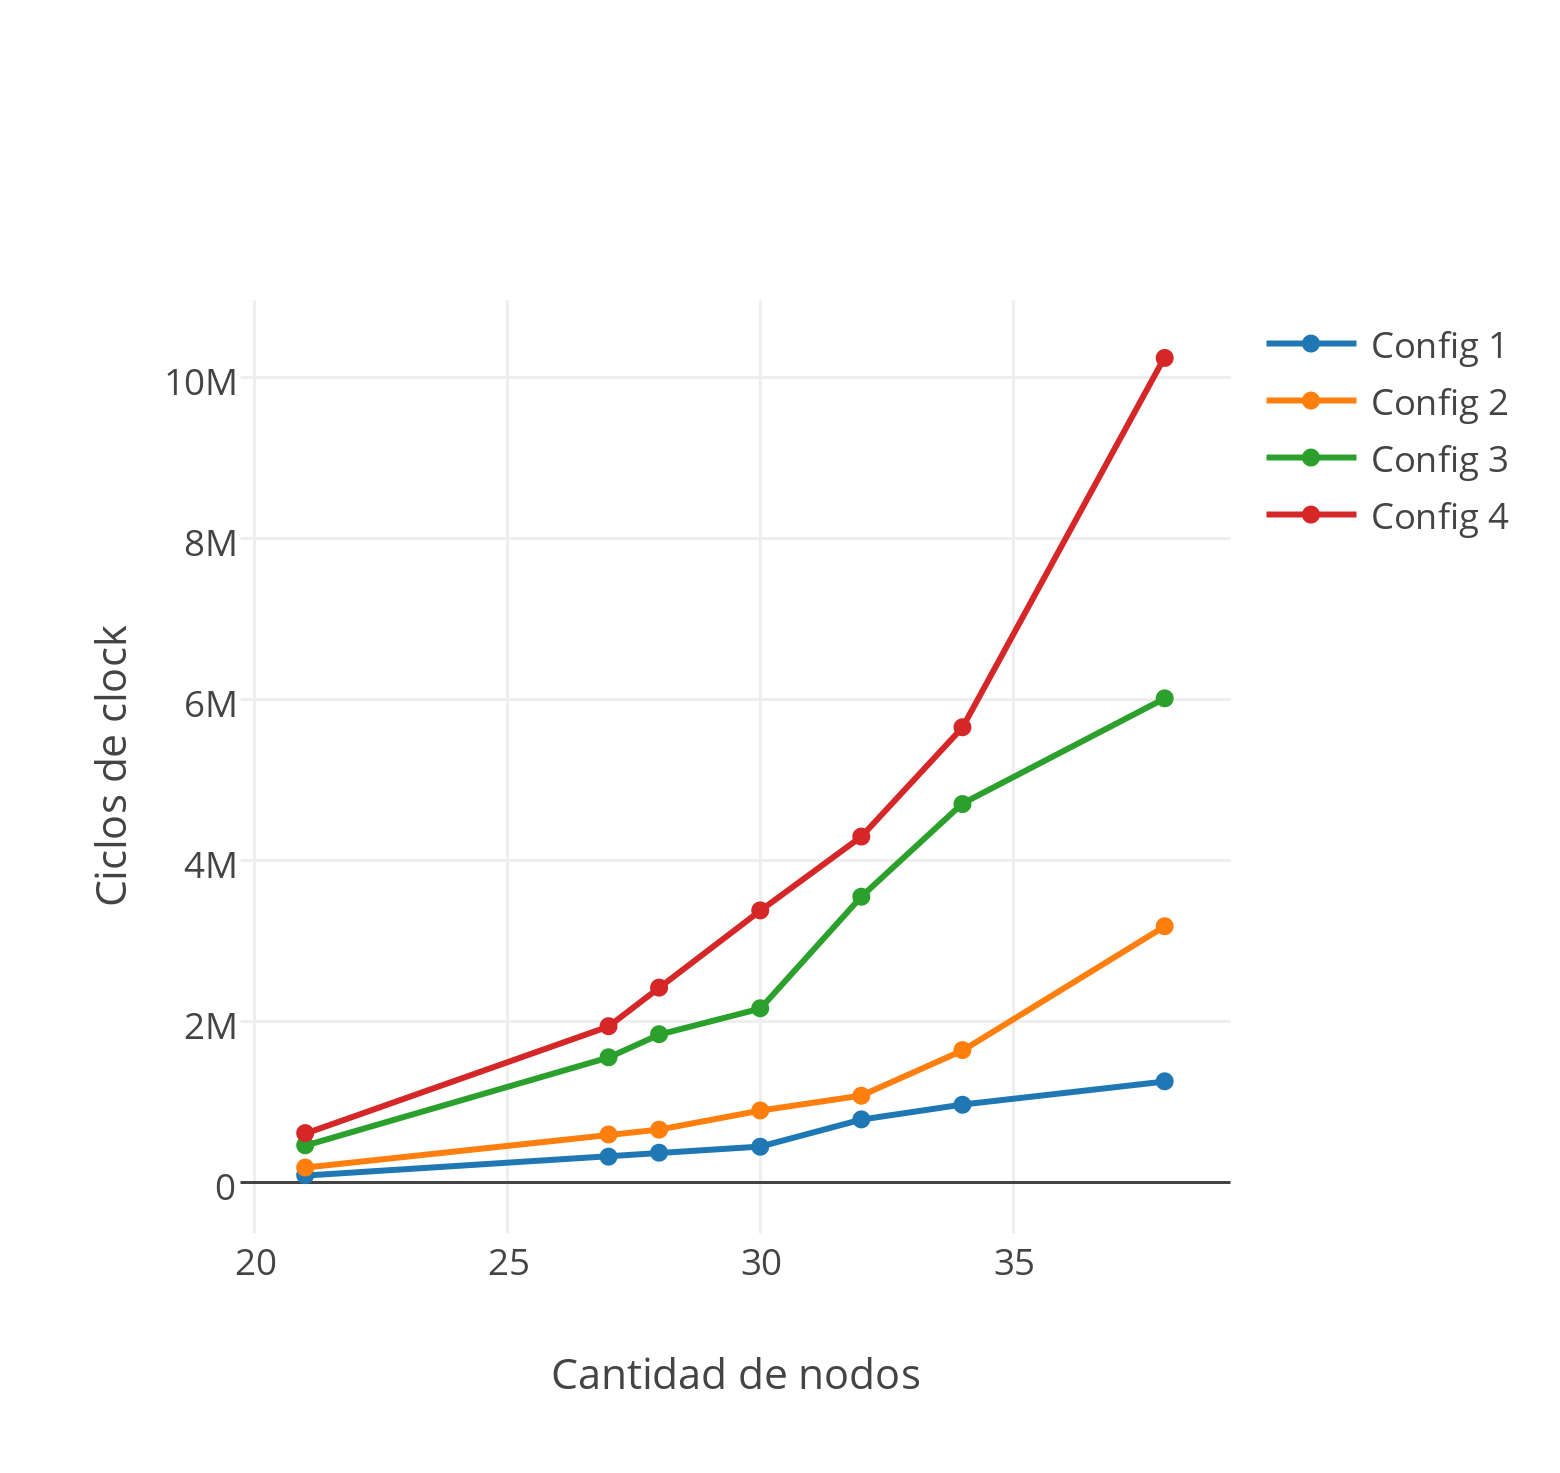
\includegraphics[scale=0.8]{imagenes/grasp-estrellas-tiempo.png}
	\end{center}
	\caption{GRASP - Estrellas}\label{fig:4B}
\end{figure}
%\FloatBarrier

\paragraph{Calidad} Se ha comparado el tamaño de la solución obtenida con el tamaño de la solución exacta. Los porcentajes de desaciertos sobre el total de instancias evaluadas son los siguientes:

\begin{verbatim}
Configuración 1: 3.34%
Configuración 2: 63.34%
Configuración 3: 0%
Configuración 4: 13.34%
\end{verbatim}

Podemos observar como la configuración 1 y 3 tienen las mejores tasas de acierto, llegando esta última a no cometer errores. Cabe destacar que la configuración 2 tiene para este tipo de grafos, un porcentaje de desaciertos muy amplio.

\subsubsection{Galaxias}

Se generaron 20 grafos $galaxia$ con entre 7 y 38 nodos.

\paragraph{Performance}

La Figura \ref{fig:4C} muestra los resultados obtenidos respecto al tiempo de ejecución. Aquí, las configuracion 1 es claramente la de mejor performance mientras que la 4 es claramente la de peor tiempo de ejecución. A priori, no podemos determinar según este gráfico quien tiene un mejor desempeño entre las configuraciones 2 y 3. 

\begin{figure}[htb]
	\begin{center}
    		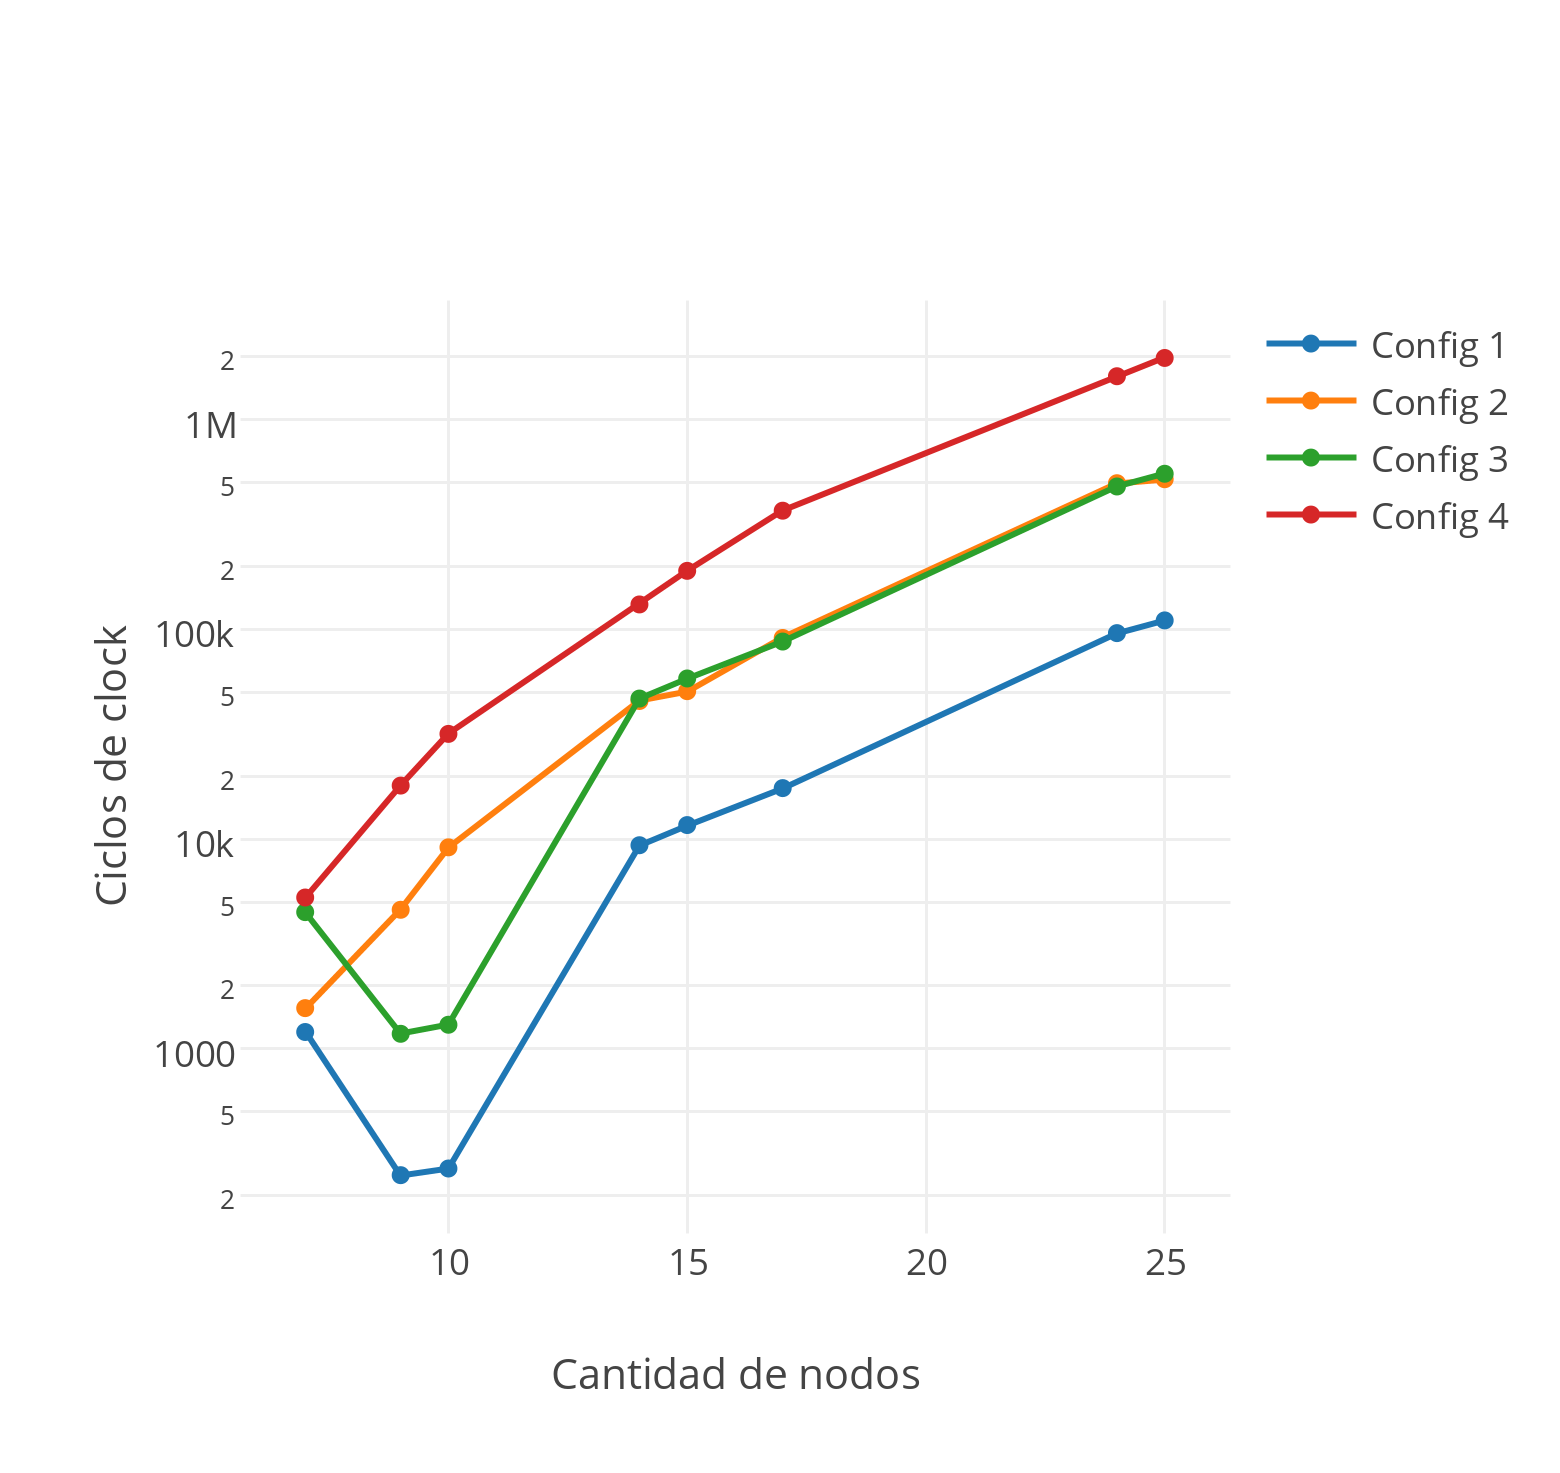
\includegraphics[scale=0.8]{imagenes/grasp-galaxias-tiempos.png}
	\end{center}
	\caption{GRASP - Galaxias}\label{fig:4C}
\end{figure}
%\FloatBarrier

\paragraph{Calidad} 
Se ha comparado el tamaño de la solución obtenida con el tamaño de la solución exacta. Los porcentajes de desaciertos sobre el total de instancias evaluadas son los siguientes:

\begin{verbatim}
Configuración 1: 0%
Configuración 2: 50%
Configuración 3: 0%
Configuración 4: 10%
\end{verbatim}

Podemos observar como las configuraciones 1 y 3 no tuvieron errores, como la configuración 4 vuelve a tener un error aceptable, y como la configuración 2 vuelve a tener una tasa de aciertos muy baja

\subsubsection{Aleatorios}

Para estos experimentos se han generado dos sets de instancias $aleatorias$. Uno contiene 120 grafos de entre 4 y 15 nodos, para poder contrastar con el algoritmo exacto (sólo se utilizara para la parte de calidad). El otro contiene 210 grafos de entre 10 y 30 nodos, que si bien no serán comparadas con el algoritmo exacto, posibilitará apreciar los tiempos de ejecución más ampliamente y tener una idea más general respecto a la calidad de las soluciones obtenidas.

\paragraph{Performance} La Figura \ref{fig:4D} muestra los resultados obtenidos respecto al tiempo de ejecución. Podemos apreciar que las configuraciones que utilizan el primer criterio de parada tienen un desempeño peor que las otras, y entre las configuraciones que utilizan el segundo criterio, la configuración 1 parecería mostrarse como la más óptima.

\begin{figure}[htb]
	\begin{center}
    		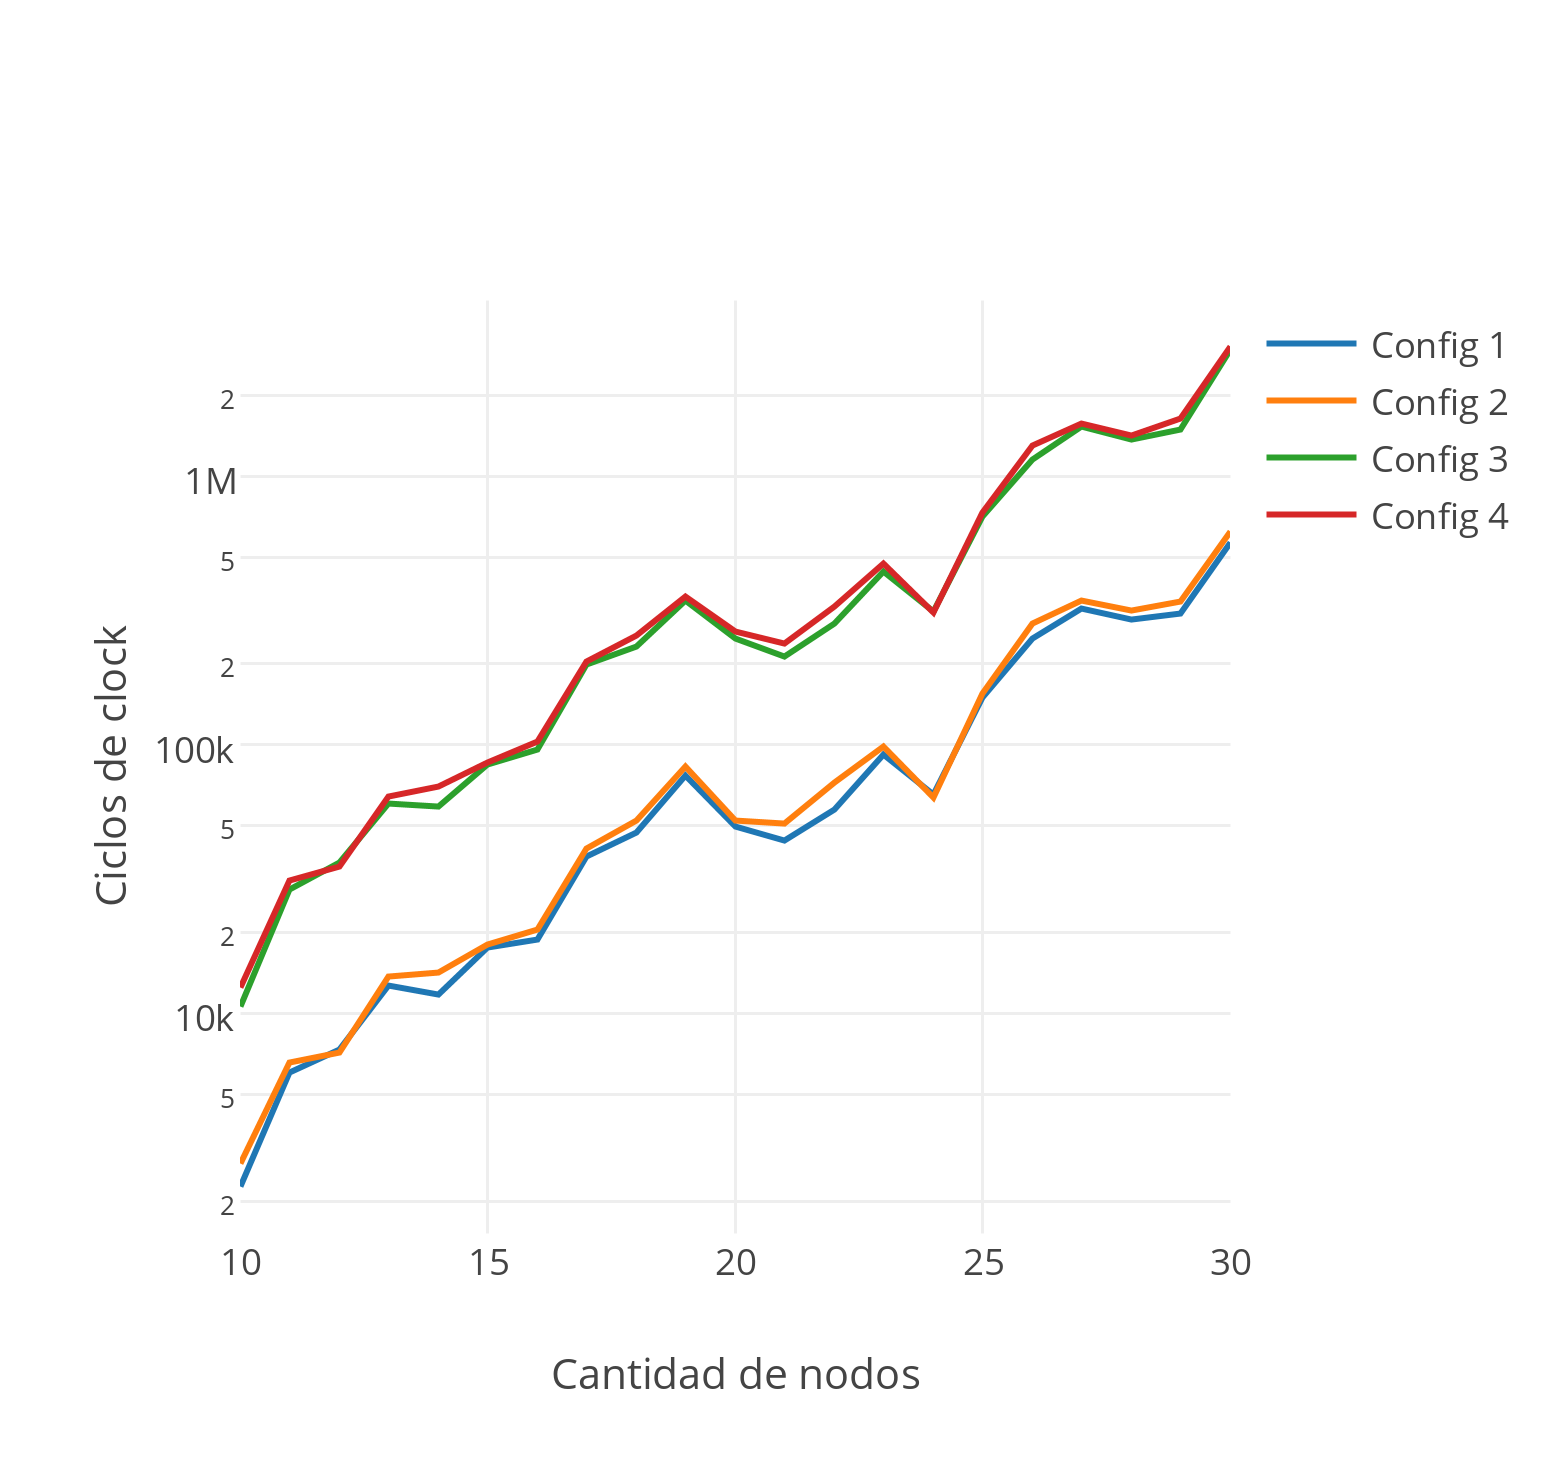
\includegraphics[scale=0.8]{imagenes/grasp-aleatorios-tiempo.png}
	\end{center}
	\caption{GRASP - Aleatorios}\label{fig:4D}
\end{figure}
%\FloatBarrier

\paragraph{Calidad} 

\subparagraph{Set 1} Se ha comparado el tamaño de la solución obtenida con el tamaño de la solución exacta.  Los porcentajes de desaciertos sobre el total de instancias evaluadas son los siguientes:

\begin{verbatim}
Configuración 1: 1.667%
Configuración 2: 0.833%
Configuración 3: 0%
Configuración 4: 0%
\end{verbatim}

Podemos observar que todas las configuraciones tienen una tasa de error muy baja, destacando la 3 y 4 que no tienen errores.

\subparagraph{Set 2} Como por el tamaño de estas instancias se dificulta la comparación con el algoritmo exacto, se consideró como la solución ``óptima'' en cada caso el menor valor obtenido entre las cuatro configuraciones, y se registró, para cada una, la cantidad de instancias en las que no se logró dicho valor. Los porcentajes de estos ``desaciertos'' sobre el total de instancias evaluadas son los siguientes:

\begin{verbatim}
Configuración 1: 1.90%
Configuración 2: 1.43%
Configuración 3: 0.48%
Configuración 4: 0.48%
\end{verbatim}

Podemos notar nuevamente como en el set 1, tasas de error muy bajas, destacando que las configuraciones 3 y 4 ahora tienen algún error.

\subsubsection{Conclusiones} 

Luego de realizar este análisis para distintas instancias, podemos observar que, en lo que respecta a la calidad de las soluciones obtenidas, la configuracion 3 es la que logra obtener mejores resultados. Cabe destacar que si bien para las familias analizadas la configuración 2 arrojo muchos desaciertos, para casos generales esto no sucede. Por otro lado, las configuraciones que utilizan el segundo criterio, requieren un tiempo de ejecución considerablemente mayor que aquellas que utilizan el primero.  Por este motivo, si bien la Configuración 3 es la que se muestra mejor en calidad, decidimos considerar a la Configuración 1 como la que mejor balancea calidad y performance. Notece, que si bien la configuración 2 tiene mejor calidad para aleatorios, configuración 1 no tiene calidad mucho peor para estos casos, tiene una considerable mejor calidad para las familias estudiadas, y es ligeramente más optimo en tiempo.
%
%\newpage
%\section{Apéndice 1: acerca de los tests}
%
%
%\subsection{Código del Problema 1}
%
%%\newpage
%\subsection{Código del Problema 2}
%
%
%
%%\newpage
%\subsection{Código del Problema 3}
%

\end{document}
